% Options for packages loaded elsewhere
\PassOptionsToPackage{unicode}{hyperref}
\PassOptionsToPackage{hyphens}{url}
%
\documentclass[
]{book}
\usepackage{amsmath,amssymb}
\usepackage{lmodern}
\usepackage{ifxetex,ifluatex}
\ifnum 0\ifxetex 1\fi\ifluatex 1\fi=0 % if pdftex
  \usepackage[T1]{fontenc}
  \usepackage[utf8]{inputenc}
  \usepackage{textcomp} % provide euro and other symbols
\else % if luatex or xetex
  \usepackage{unicode-math}
  \defaultfontfeatures{Scale=MatchLowercase}
  \defaultfontfeatures[\rmfamily]{Ligatures=TeX,Scale=1}
\fi
% Use upquote if available, for straight quotes in verbatim environments
\IfFileExists{upquote.sty}{\usepackage{upquote}}{}
\IfFileExists{microtype.sty}{% use microtype if available
  \usepackage[]{microtype}
  \UseMicrotypeSet[protrusion]{basicmath} % disable protrusion for tt fonts
}{}
\makeatletter
\@ifundefined{KOMAClassName}{% if non-KOMA class
  \IfFileExists{parskip.sty}{%
    \usepackage{parskip}
  }{% else
    \setlength{\parindent}{0pt}
    \setlength{\parskip}{6pt plus 2pt minus 1pt}}
}{% if KOMA class
  \KOMAoptions{parskip=half}}
\makeatother
\usepackage{xcolor}
\IfFileExists{xurl.sty}{\usepackage{xurl}}{} % add URL line breaks if available
\IfFileExists{bookmark.sty}{\usepackage{bookmark}}{\usepackage{hyperref}}
\hypersetup{
  pdftitle={AMAT- Ciencia de Datos y Machine Learning 2},
  pdfauthor={Karina Lizette Gamboa Puente; Oscar Arturo Bringas López},
  hidelinks,
  pdfcreator={LaTeX via pandoc}}
\urlstyle{same} % disable monospaced font for URLs
\usepackage{color}
\usepackage{fancyvrb}
\newcommand{\VerbBar}{|}
\newcommand{\VERB}{\Verb[commandchars=\\\{\}]}
\DefineVerbatimEnvironment{Highlighting}{Verbatim}{commandchars=\\\{\}}
% Add ',fontsize=\small' for more characters per line
\usepackage{framed}
\definecolor{shadecolor}{RGB}{248,248,248}
\newenvironment{Shaded}{\begin{snugshade}}{\end{snugshade}}
\newcommand{\AlertTok}[1]{\textcolor[rgb]{0.94,0.16,0.16}{#1}}
\newcommand{\AnnotationTok}[1]{\textcolor[rgb]{0.56,0.35,0.01}{\textbf{\textit{#1}}}}
\newcommand{\AttributeTok}[1]{\textcolor[rgb]{0.77,0.63,0.00}{#1}}
\newcommand{\BaseNTok}[1]{\textcolor[rgb]{0.00,0.00,0.81}{#1}}
\newcommand{\BuiltInTok}[1]{#1}
\newcommand{\CharTok}[1]{\textcolor[rgb]{0.31,0.60,0.02}{#1}}
\newcommand{\CommentTok}[1]{\textcolor[rgb]{0.56,0.35,0.01}{\textit{#1}}}
\newcommand{\CommentVarTok}[1]{\textcolor[rgb]{0.56,0.35,0.01}{\textbf{\textit{#1}}}}
\newcommand{\ConstantTok}[1]{\textcolor[rgb]{0.00,0.00,0.00}{#1}}
\newcommand{\ControlFlowTok}[1]{\textcolor[rgb]{0.13,0.29,0.53}{\textbf{#1}}}
\newcommand{\DataTypeTok}[1]{\textcolor[rgb]{0.13,0.29,0.53}{#1}}
\newcommand{\DecValTok}[1]{\textcolor[rgb]{0.00,0.00,0.81}{#1}}
\newcommand{\DocumentationTok}[1]{\textcolor[rgb]{0.56,0.35,0.01}{\textbf{\textit{#1}}}}
\newcommand{\ErrorTok}[1]{\textcolor[rgb]{0.64,0.00,0.00}{\textbf{#1}}}
\newcommand{\ExtensionTok}[1]{#1}
\newcommand{\FloatTok}[1]{\textcolor[rgb]{0.00,0.00,0.81}{#1}}
\newcommand{\FunctionTok}[1]{\textcolor[rgb]{0.00,0.00,0.00}{#1}}
\newcommand{\ImportTok}[1]{#1}
\newcommand{\InformationTok}[1]{\textcolor[rgb]{0.56,0.35,0.01}{\textbf{\textit{#1}}}}
\newcommand{\KeywordTok}[1]{\textcolor[rgb]{0.13,0.29,0.53}{\textbf{#1}}}
\newcommand{\NormalTok}[1]{#1}
\newcommand{\OperatorTok}[1]{\textcolor[rgb]{0.81,0.36,0.00}{\textbf{#1}}}
\newcommand{\OtherTok}[1]{\textcolor[rgb]{0.56,0.35,0.01}{#1}}
\newcommand{\PreprocessorTok}[1]{\textcolor[rgb]{0.56,0.35,0.01}{\textit{#1}}}
\newcommand{\RegionMarkerTok}[1]{#1}
\newcommand{\SpecialCharTok}[1]{\textcolor[rgb]{0.00,0.00,0.00}{#1}}
\newcommand{\SpecialStringTok}[1]{\textcolor[rgb]{0.31,0.60,0.02}{#1}}
\newcommand{\StringTok}[1]{\textcolor[rgb]{0.31,0.60,0.02}{#1}}
\newcommand{\VariableTok}[1]{\textcolor[rgb]{0.00,0.00,0.00}{#1}}
\newcommand{\VerbatimStringTok}[1]{\textcolor[rgb]{0.31,0.60,0.02}{#1}}
\newcommand{\WarningTok}[1]{\textcolor[rgb]{0.56,0.35,0.01}{\textbf{\textit{#1}}}}
\usepackage{longtable,booktabs,array}
\usepackage{calc} % for calculating minipage widths
% Correct order of tables after \paragraph or \subparagraph
\usepackage{etoolbox}
\makeatletter
\patchcmd\longtable{\par}{\if@noskipsec\mbox{}\fi\par}{}{}
\makeatother
% Allow footnotes in longtable head/foot
\IfFileExists{footnotehyper.sty}{\usepackage{footnotehyper}}{\usepackage{footnote}}
\makesavenoteenv{longtable}
\usepackage{graphicx}
\makeatletter
\def\maxwidth{\ifdim\Gin@nat@width>\linewidth\linewidth\else\Gin@nat@width\fi}
\def\maxheight{\ifdim\Gin@nat@height>\textheight\textheight\else\Gin@nat@height\fi}
\makeatother
% Scale images if necessary, so that they will not overflow the page
% margins by default, and it is still possible to overwrite the defaults
% using explicit options in \includegraphics[width, height, ...]{}
\setkeys{Gin}{width=\maxwidth,height=\maxheight,keepaspectratio}
% Set default figure placement to htbp
\makeatletter
\def\fps@figure{htbp}
\makeatother
\setlength{\emergencystretch}{3em} % prevent overfull lines
\providecommand{\tightlist}{%
  \setlength{\itemsep}{0pt}\setlength{\parskip}{0pt}}
\setcounter{secnumdepth}{5}
\usepackage{booktabs}
\usepackage{booktabs}
\usepackage{longtable}
\usepackage{array}
\usepackage{multirow}
\usepackage{wrapfig}
\usepackage{float}
\usepackage{colortbl}
\usepackage{pdflscape}
\usepackage{tabu}
\usepackage{threeparttable}
\usepackage{threeparttablex}
\usepackage[normalem]{ulem}
\usepackage{makecell}
\usepackage{xcolor}
\ifluatex
  \usepackage{selnolig}  % disable illegal ligatures
\fi
\usepackage[]{natbib}
\bibliographystyle{apalike}

\title{AMAT- Ciencia de Datos y Machine Learning 2}
\author{Karina Lizette Gamboa Puente \and Oscar Arturo Bringas López}
\date{}

\begin{document}
\maketitle

{
\setcounter{tocdepth}{1}
\tableofcontents
}
\hypertarget{bienvenida}{%
\chapter{BIENVENIDA}\label{bienvenida}}

\hypertarget{objetivo}{%
\section{Objetivo}\label{objetivo}}

Desarrollar conocimiento y habilidades para implementar modelos complejos de Machine Learning a través de un flujo de trabajo limpio, ordenado y sistematizado a mediante las librerías en \emph{R} más novedosas que han sido desarrolladas hasta el momento. Al finalizar este curso, el participante será capáz de combinar distintas clases de modelos para dar una solución compleja y precisa a problemas predictivos. Aprenderá a cuantificar los problemas éticos asociados al sesgo o inequidad producidos por modelos de machine learning, así como su interpretación en el mundo productivo. Finalmente, se estudiará la manera de desarrollar un diseño de experimento para implementarse en el ámbito empresarial de modo que el participante pueda tomar mejores decisiones para contribuir en su ambiente laboral.

\textbf{Se asume que el alumno tiene conocimientos generales de estadística, bases matemáticas y de programación básica en R y que cuenta con los conocimientos teóricos básicos de machine learning y prácticos con tidymodels.}

\hypertarget{instructores}{%
\section{Instructores}\label{instructores}}

\textbf{ACT. ARTURO BRINGAS}

\textbf{LinkedIn:} \href{https://www.linkedin.com/in/arturo-bringas/}{arturo-bringas}
\textbf{Email:} \href{mailto:act.arturo.b@ciencias.unam.mx}{\nolinkurl{act.arturo.b@ciencias.unam.mx}}

Actuario, egresado de la Facultad de Ciencias y Maestría en Ciencia de Datos, ITAM.
Experiencia en modelos predictivos y de clasificación de machine learning aplicado a seguros, deportes y movilidad internacional. Es jefe de departamento en Investigación Aplicada y Opinión de la UNAM, donde realiza estudios estadísticos de impacto social. Es consultor para empresas y organizaciones como GNP, El Universal, UNAM, Sinnia, la Organización de las Naciones Unidas Contra la Droga y el Delito (UNODC), entre otros. Actualmente es profesor de \emph{ciencia de datos y machine learning} en AMAT y se desempeña como consultor independiente en diferentes proyectos contribuyendo a empresas en temas de machine learning, estadística, series de tiempo, visualización de datos y análisis geoespacial.

\begin{center}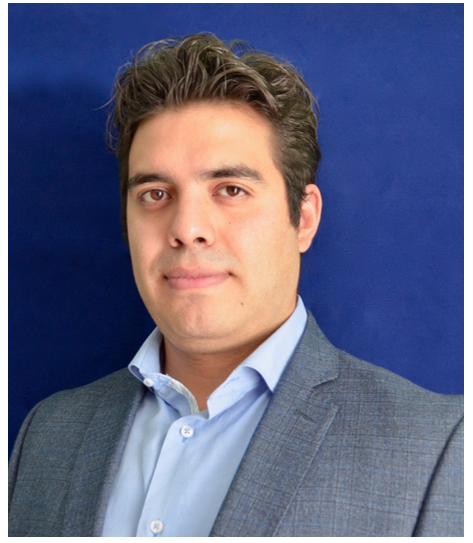
\includegraphics{img/00-presentacion/arturo} \end{center}

\textbf{ACT. KARINA LIZETTE GAMBOA}

\textbf{LinkedIn:} \href{https://www.linkedin.com/in/kalizzygam/}{KaLizzyGam}
\textbf{Email:} \href{mailto:lizzygamboa@ciencias.unam.mx}{\nolinkurl{lizzygamboa@ciencias.unam.mx}}

Actuaria, egresada de la Facultad de Ciencias, UNAM, candidata a Maestra en
Ciencia de Datos por el ITAM.

Experiencia en áreas de analítica predictiva e inteligencia del negocio. Lead y Senior
Data Scientist en consultoría en diferentes sectores como tecnología, asegurador,
financiero y bancario. Experta en entendimiento de negocio para la correcta
implementación de algoritmos de inteligencia y explotación de datos.
Actualmente se desarrolla como Arquitecta de Soluciones Analíticas en Merama,
startup mexicana clasificada como uno de los nuevos unicornios de Latinoamérica.
Senior Data Science en CLOSTER y como profesora del diplomado de Metodología
de la Investigación Social por la UNAM así como instructora de cursos de Ciencia de
Datos en AMAT.

Empresas anteriores: GNP, Activer Banco y Casa de Bolsa, PlayCity Casinos,
RakenDataGroup Consulting, entre otros.

\begin{center}
\includegraphics[width=600pt]{img/00-presentacion/lizzy} \end{center}

\hypertarget{ciencia-de-datos-en-r}{%
\section{Ciencia de Datos en R}\label{ciencia-de-datos-en-r}}

\begin{center}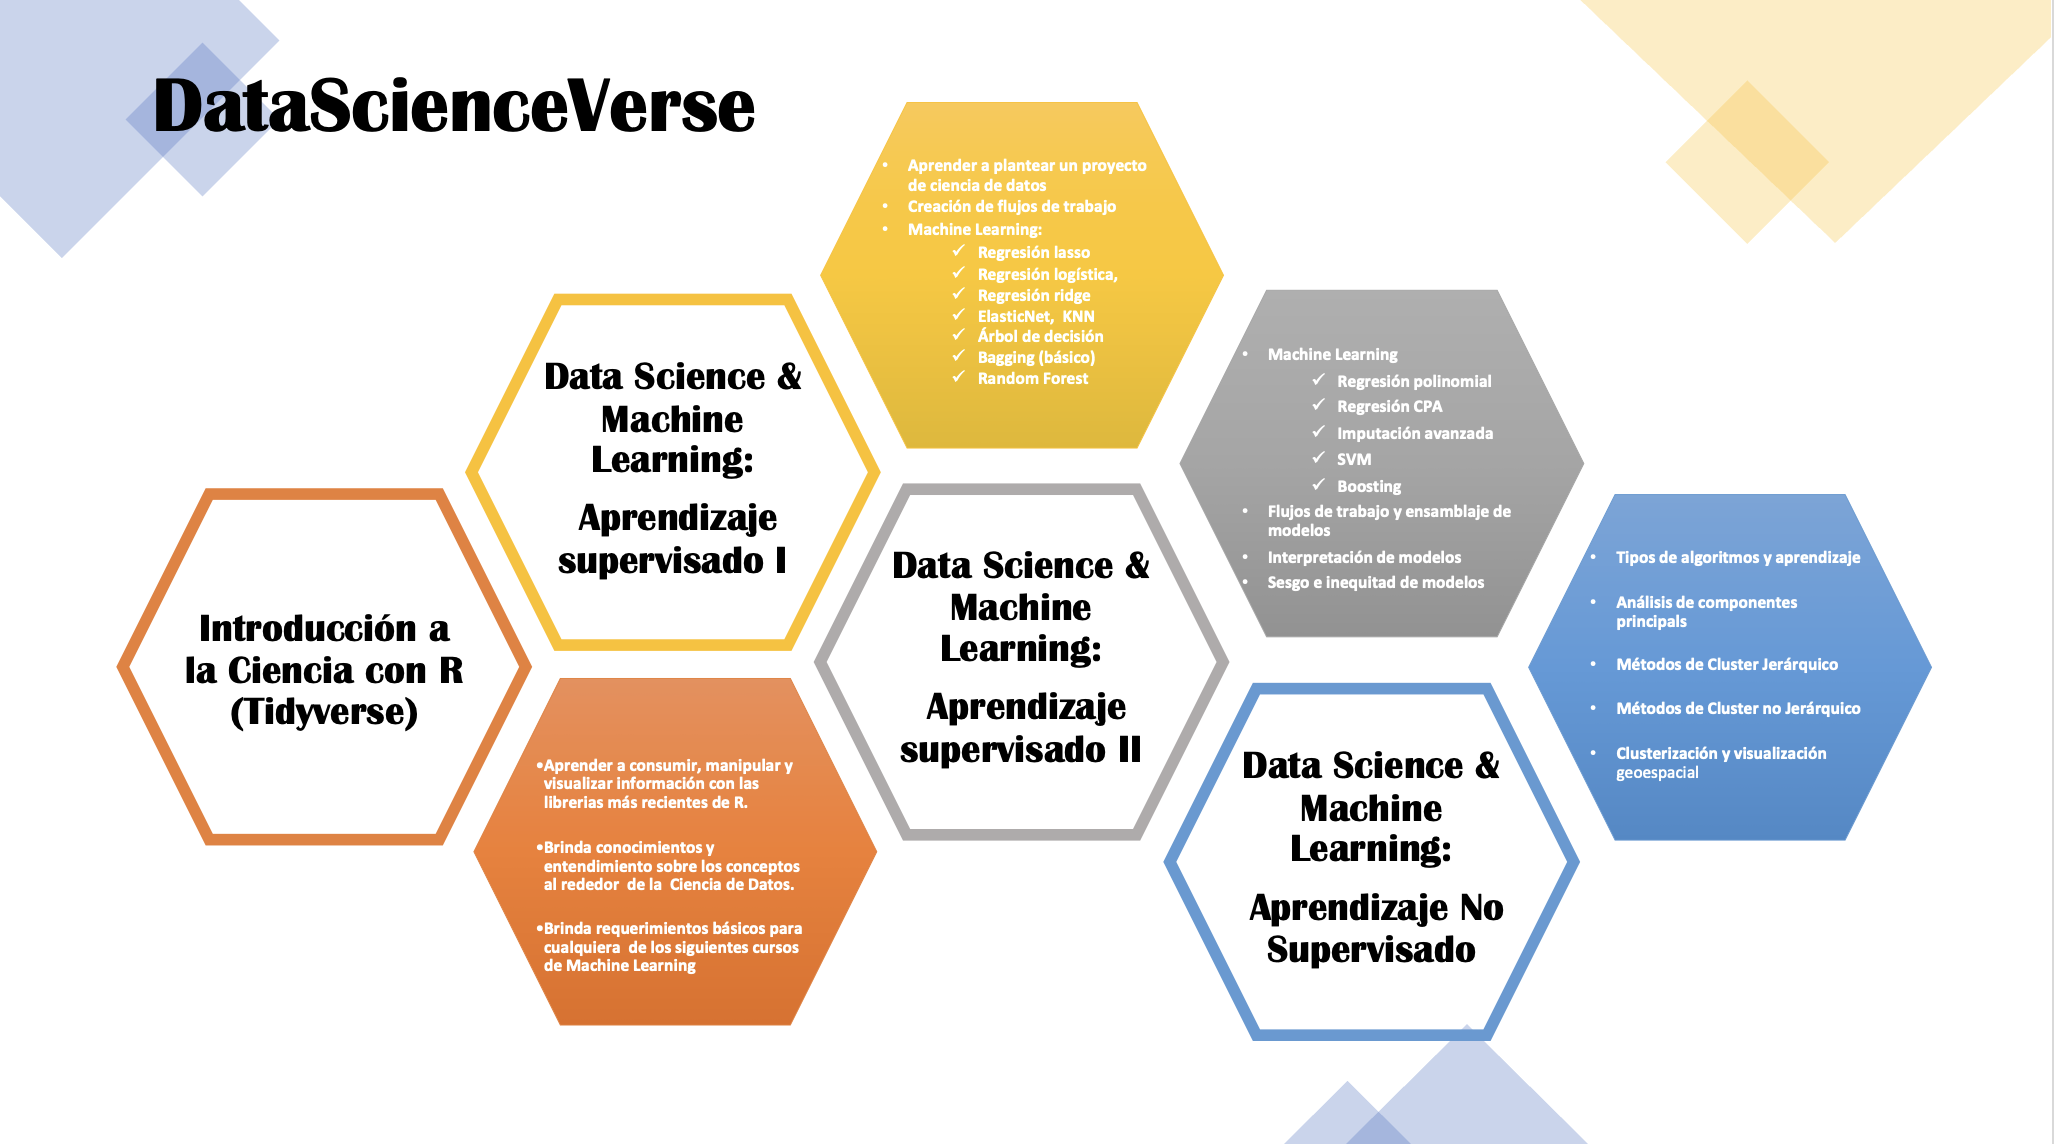
\includegraphics[width=600pt]{img/00-presentacion/DataScienceVerse} \end{center}

\hypertarget{estructura-del-curso-actual}{%
\section{Estructura del curso actual}\label{estructura-del-curso-actual}}

\hypertarget{alcances-del-curso}{%
\subsection{Alcances del curso}\label{alcances-del-curso}}

Al finalizar el módulo, el participante sabrá plantear un proyecto de ciencia de datos, desde sus requerimientos hasta sus implementación comercial. Sabrá crear flujos de trabajo limpios y ordenados para crear poderosos modelos de Machine Learning. Podrá comparar múltiples modelos y seleccionar el que más aportación realice a su negocio considerando la ética alrededor del sesgo e inequidad producida por modelos. Profundizará su conocimiento en la interpretación de modelos complejos y aprenderá a cuantificar el beneficio comercial de la implementación de modelos.

\textbf{Requisitos:}

\begin{quote}
Computadora con al menos 4Gb Ram.
\end{quote}

\begin{quote}
Instalación de R con al menos versión 4.1.0
\end{quote}

\begin{quote}
Instalación de Rstudio con al menos versión 1.4
\end{quote}

\begin{quote}
Data Science \& Machine Learning (Aprendizaje Supervisado I)
\end{quote}

\textbf{Temario:}

\textbf{1.- Machine Learning (10 HRS)}

\begin{itemize}
\tightlist
\item
  Regresión polinomial
\item
  Regresión con CPA
\item
  Imputación
\item
  SVM
\item
  Boosting
\end{itemize}

\textbf{2. Flujos de trabajo y ensamblajes (8 HRS)}

\begin{itemize}
\tightlist
\item
  Pipelines
\item
  Workflowsets
\item
  Comparación de modelos
\item
  Stacking
\end{itemize}

\textbf{3. Sesgo e inequidad de modelos (4 HRS)}

\begin{itemize}
\tightlist
\item
  Cuantificación de sesgo
\item
  Cuantificación de inequidad
\end{itemize}

\textbf{4. Interpretación de modelos (4 HRS)}

\begin{itemize}
\tightlist
\item
  LIME
\item
  ghv
\end{itemize}

\textbf{5. Aplicación a negocios (6 HRS)}

\begin{itemize}
\tightlist
\item
  Diseño de experimentos en campañas de retención
\item
  Valuación de implementación de modelos
\end{itemize}

\hypertarget{duraciuxf3n-y-evaluaciuxf3n-del-curso}{%
\section{Duración y evaluación del curso}\label{duraciuxf3n-y-evaluaciuxf3n-del-curso}}

\begin{itemize}
\item
  El programa tiene una duración de 32 hrs.
\item
  Las clases serán impartidas los días domingo, de 9:00 am a 1:00 pm
\item
  Serán asignados ejercicios que el participante deberá resolver entre una semana y otra.
\item
  Al final del curso se solicitará un proyecto final, el cual \textbf{deberá ser entregado para ser acreedor a la constancia de participación}.
\end{itemize}

\hypertarget{recursos-y-dinuxe1mica-de-clase}{%
\section{Recursos y dinámica de clase}\label{recursos-y-dinuxe1mica-de-clase}}

En esta clase estaremos usando:

\begin{itemize}
\tightlist
\item
  R \href{https://cran.r-project.org/}{da click aquí si aún no lo descargas}
\item
  RStudio \href{https://www.rstudio.com/products/rstudio/download/}{da click aquí también}
\item
  Miro \href{https://miro.com/welcomeonboard/c3huendzNURhRUVGbHlsWGVFYlBBMXRaSncybXRrbjBRU2R5WWg2eDFKUXY1VlJ1SGJFdmc4ZmRuWEgwcllpenwzMDc0NDU3MzYxMzQwNDIyODEy?invite_link_id=152058640259}{úsame}
\item
  Zoom \href{https://us02web.zoom.us/j/5155440751?pwd=YzJCOGF0VnlZdlZlS0Fpc3MvZEhadz09}{Clases}

  \begin{itemize}
  \tightlist
  \item
    Pulgar arriba: Voy bien, estoy entendiendo!
  \item
    Pulgar abajo: Eso no quedó muy claro
  \item
    Mano arriba: Quiero participar/preguntar ó Ya estoy listo para iniciar
  \end{itemize}
\item
  Grupo de WhatsApp \href{}{El chismecito está aquí}
\item
  \href{}{Google Drive}
\item
  Notas de clase \href{https://acturio.github.io/amt22_03intro2mls2/}{Revisame si quieres aprender}
\end{itemize}

\hypertarget{repaso}{%
\chapter{Repaso}\label{repaso}}

En los cursos anteriores, hemos hablando a cerca del proceso completo de Ciencia de Datos, para poder empezar con la segunda parte del curso de Analisis Supervisado, valele la pena hacer un breve repaso de lo que hemos estudiado hasta el momento.

\hypertarget{machine-learning}{%
\section{Machine Learning}\label{machine-learning}}

\textbf{Machine Learning} o --aprendizaje automático-- es una rama de la inteligencia artificial que permite que las máquinas aprendan de los patrones existentes en los datos. Se usan métodos computacionales para aprender de datos con el fin de producir reglas para mejorar el desempeño en alguna tarea o toma de decisión. (Está enfocado en la programación de máquinas para aprender de los patrones existentes en datos principalmente estructurados y anticiparse al futuro)

\begin{center}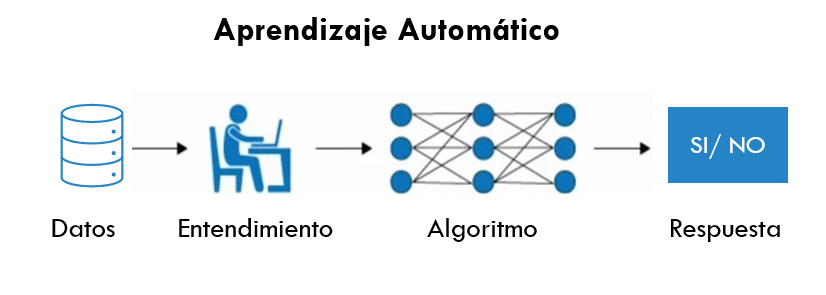
\includegraphics[width=600pt]{img/01-repaso/02_ml} \end{center}

\begin{center}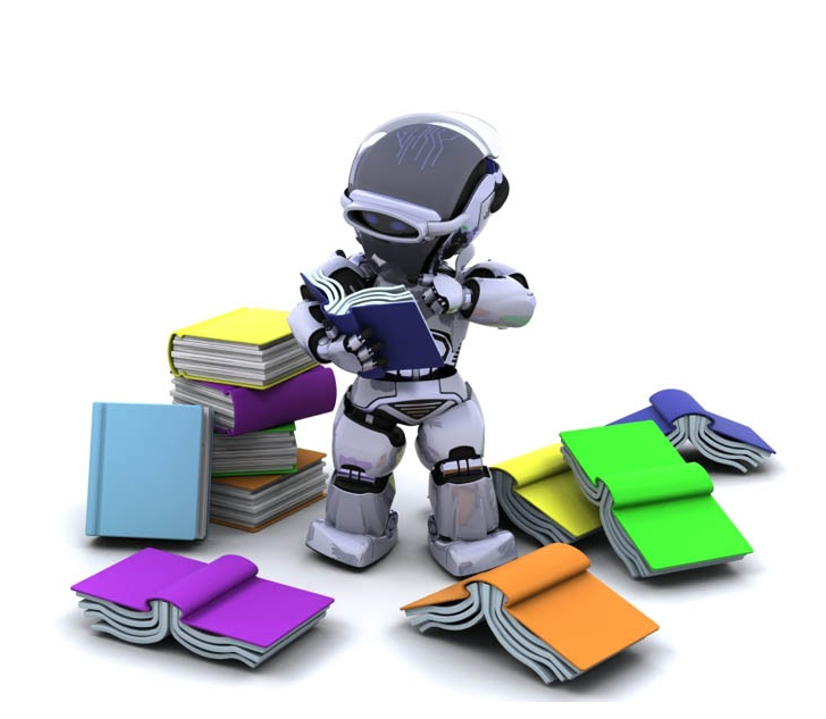
\includegraphics[width=600pt]{img/01-repaso/03_supervisado_robo} \end{center}

\hypertarget{tipos-de-aprendizaje}{%
\section{Tipos de aprendizaje}\label{tipos-de-aprendizaje}}

Platicamos en el módulo pasado que al hablar de Machine Learning, existen distintos tipos de aprendizaje, siendo los más comúnes:

\begin{itemize}
\tightlist
\item
  Aprendizaje supervisado
\item
  Aprendizaje no supervisado
\end{itemize}

Otreos ejemplos de especialidades son

\begin{itemize}
\tightlist
\item
  Aprendizaje profundo
\item
  Aprendizaje por refuerzo
\end{itemize}

La diferencia entre el análisis supervisado y el no supervisado es la etiqueta, es decir, en el análisis supervisado tenemos una etiqueta ``correcta'' y el objetivo de los algoritmos es predecir esta etiqueta.

\hypertarget{aprendizaje-supervisado}{%
\subsection{Aprendizaje supervisado}\label{aprendizaje-supervisado}}

\begin{itemize}
\item
  Conocemos la respuesta correcta de antemano.
\item
  Esta respuesta correcta fue ``etiquetada'' por un humano (la mayoría de las veces, en algunas circunstancias puede ser generada por otro algoritmo).
\item
  Debido a que conocemos la respuesta correcta, existen muchas métricas de desempeño del modelo para verificar que nuestro algoritmo está haciendo las cosas ``bien''.
\end{itemize}

\hypertarget{tipos-de-aprendizaje-supervisado-regresiuxf3n-vs-clasificaciuxf3n}{%
\subsubsection{Tipos de aprendizaje supervisado (Regresión vs clasificación)}\label{tipos-de-aprendizaje-supervisado-regresiuxf3n-vs-clasificaciuxf3n}}

Existen dos tipos principales de aprendizaje supervisado, esto depende del tipo de la variable respuesta:

\begin{itemize}
\item
  Los algoritmos de \textbf{clasificación} se usan cuando el resultado deseado es una etiqueta discreta, es decir, clasifican un elemento dentro de diversas clases.
\item
  En un problema de \textbf{regresión}, la variable target o variable a predecir es un valor numérico.
\end{itemize}

\begin{center}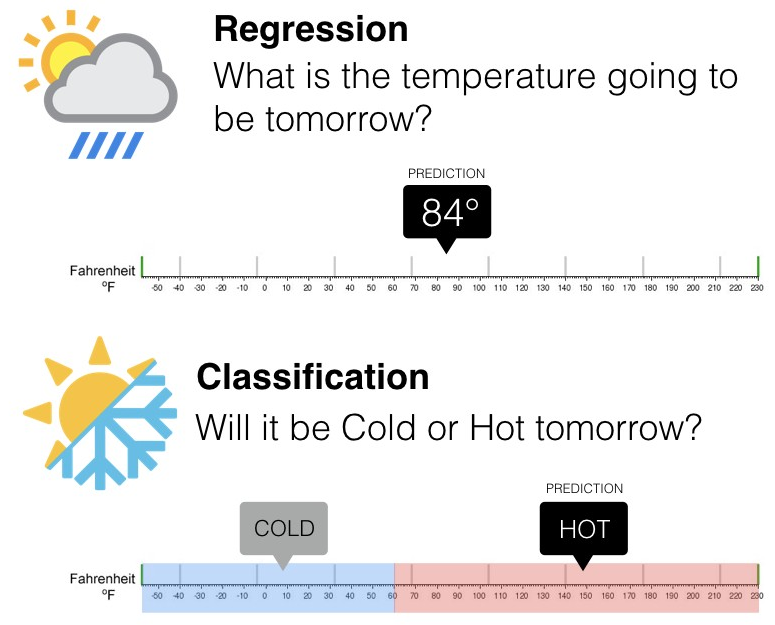
\includegraphics[width=700pt,height=450pt]{img/01-repaso/13_regresion_clasificacion} \end{center}

\hypertarget{aprendizaje-no-supervisado}{%
\subsection{Aprendizaje no supervisado}\label{aprendizaje-no-supervisado}}

\begin{itemize}
\item
  Aquí no tenemos la respuesta correcta de antemano ¿cómo podemos saber que el algoritmo está bien o mal?
\item
  Estadísticamente podemos verificar que el algoritmo está bien
\item
  Siempre tenemos que verificar con el cliente si los resultados que estamos obteniendo tienen sentido de negocio. Por ejemplo, número de grupos y características
\end{itemize}

\begin{center}
\includegraphics{img/01-repaso/14_nosupervisado_robo} \end{center}

\hypertarget{el-proceso-de-machine-learning}{%
\section{El proceso de Machine Learning}\label{el-proceso-de-machine-learning}}

La cuestión no es solo saber para qué sirve el Machine Learning, sino que saber cómo funciona y cómo poder implementarlo en la industria para aprovecharse de sus beneficios.
Hay ciertos pasos que usualmente se siguen para crear un modelo de Machine Learning. Estos son típicamente realizados por científicos de los datos que trabajan en estrecha colaboración con los profesionales de los negocios para los que se está desarrollando el modelo.

\begin{enumerate}
\def\labelenumi{\arabic{enumi}.}
\tightlist
\item
  \textbf{Seleccionar y preparar un conjunto de datos de entrenamiento}:
  Los \textbf{datos de entrenamiento} son un conjunto de datos representativos de los datos que el modelo de Machine Learning ingerirá para resolver el problema que está diseñado para resolver.
  Los datos de entrenamiento deben prepararse adecuadamente: aleatorizados y comprobados en busca de desequilibrios o sesgos que puedan afectar al entrenamiento. También deben dividirse en dos subconjuntos: el \textbf{subconjunto de entrenamiento}, que se utilizará para entrenar el algoritmo, y el \textbf{subconjunto de validación}, que se utilizará para probarlo y perfeccionarlo.
\end{enumerate}

\begin{center}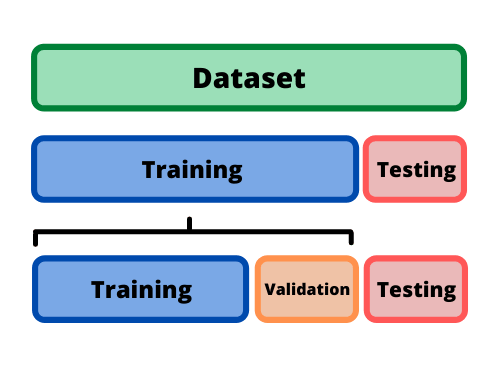
\includegraphics[width=600pt]{img/01-repaso/train-and-test} \end{center}

\begin{enumerate}
\def\labelenumi{\arabic{enumi}.}
\setcounter{enumi}{1}
\item
  \textbf{Elegir un algoritmo para ejecutarlo en el conjunto de datos de entrenamiento}:
  Este es uno de los pasos más importantes, ya que se debe elegir qué algoritmo utilizar, siendo este un conjunto de pasos de procesamiento estadístico. El tipo de algoritmo depende del tipo (supervisado o no supervisado), la cantidad de datos del conjunto de datos de entrenamiento y del tipo de problema que se debe resolver.
\item
  \textbf{Entrenamiento del algoritmo para crear el modelo}:
  El entrenamiento del algoritmo es un proceso iterativo: implica ejecutar las variables a través del algoritmo, comparar el resultado con los resultados que debería haber producido, ajustar los pesos y los sesgos dentro del algoritmo que podrían dar un resultado más exacto, y ejecutar las variables de nuevo hasta que el algoritmo devuelva el resultado correcto la mayoría de las veces. El algoritmo resultante, entrenado y preciso, es el modelo de Machine Learning.
\item
  \textbf{Usar y mejorar el modelo}:
  El paso final es utilizar el modelo con nuevos datos y, en el mejor de los casos, para que mejore en precisión y eficacia con el tiempo. De dónde procedan los nuevos datos dependerá del problema que se resuelva. Por ejemplo, un modelo de Machine Learning diseñado para identificar el spam ingerirá mensajes de correo electrónico, mientras que un modelo de Machine Learning que maneja una aspiradora robot ingerirá datos que resulten de la interacción en el mundo real con muebles movidos o nuevos objetos en la habitación.
\end{enumerate}

\hypertarget{errores-sesgo-vs-varianza}{%
\section{Errores: Sesgo vs varianza}\label{errores-sesgo-vs-varianza}}

En el mundo de Machine Learning cuando desarrollamos un modelo nos esforzamos para hacer que sea lo más preciso, ajustando los parámetros, pero la realidad es que no se puede construir un modelo 100\% preciso ya que nunca pueden estar libres de errores.

Comprender cómo las diferentes fuentes de error generan sesgo y varianza nos ayudará a mejorar el proceso de ajuste de datos, lo que resulta en modelos más precisos, adicionalmente también evitará el error de sobreajuste y falta de ajuste.

\begin{itemize}
\tightlist
\item
  \textbf{Error por sesgo:}
\end{itemize}

Es la diferencia entre la predicción esperada de nuestro modelo y los valores verdaderos. Aunque al final nuestro objetivo es siempre construir modelos que puedan predecir datos muy cercanos a los valores verdaderos, no siempre es tan fácil porque algunos algoritmos son simplemente demasiado rígidos para aprender señales complejas del conjunto de datos.

Imagina ajustar una regresión lineal a un conjunto de datos que tiene un patrón no lineal, no importa cuántas observaciones más recopiles, una regresión lineal no podrá modelar las curvas en esos datos. Esto se conoce como \emph{underfitting}.

\begin{itemize}
\tightlist
\item
  \textbf{Error por varianza:}
\end{itemize}

Se refiere a la cantidad que la estimación de la función objetivo cambiará si se utiliza diferentes datos de entrenamiento. La función objetivo se estima a partir de los datos de entrenamiento mediante un algoritmo de Machine Learning, por lo que deberíamos esperar que el algoritmo tenga alguna variación. Idealmente no debería cambiar demasiado de un conjunto de datos de entrenamiento a otro.

\begin{center}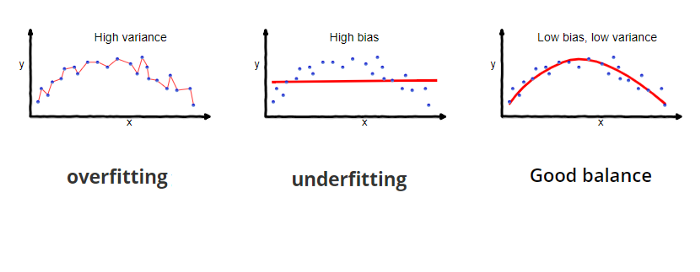
\includegraphics[width=650pt,height=350pt]{img/01-repaso/3-1-3-biasvar} \end{center}

Los algoritmos de Machine Learning que tienen una gran varianza están fuertemente influenciados por los detalles de los datos de entrenamiento, esto significa que los detalles de la capacitación influyen en el número y los tipos de parámetros utilizados para caracterizar la función de mapeo.

\begin{itemize}
\tightlist
\item
  \textbf{Error irreducible:}
  El error irreducible no se puede reducir, independientemente de qué algoritmo se usa. También se le conoce como ruido y, por lo general, proviene por factores como variables desconocidas que influyen en el mapeo de las variables de entrada a la variable de salida, un conjunto de características incompleto o un problema mal enmarcado. Acá es importante comprender que no importa cuán bueno hagamos nuestro modelo, nuestros datos tendrán cierta cantidad de ruido o un error irreductible que no se puede eliminar.
\end{itemize}

\hypertarget{ingenieruxeda-de-caracteruxedsticas-feature-engineering}{%
\section{Ingeniería de características (Feature Engineering)}\label{ingenieruxeda-de-caracteruxedsticas-feature-engineering}}

La ingenería de datos y procesamiento de datos es parte vital del desarrollo de un buen modelo.

En este curso analizaremos distintos métodos de machine learning que permitirán predecir una respuesta numérica o categórica. Usaremos el lenguaje de programación \emph{R} para dicho procesamiento.

\begin{center}\rule{0.5\linewidth}{0.5pt}\end{center}

Hay varios pasos que se deben de seguir para crear un modelo útil:

\begin{itemize}
\tightlist
\item
  Recopilación de datos.
\item
  Limpieza de datos.
\item
  Creación de nuevas variables.
\item
  Estimación de parámetros.
\item
  Selección y ajuste del modelo.
\item
  Evaluación del rendimiento.
\end{itemize}

Al comienzo de un proyecto, generalmente hay un conjunto finito de datos disponibles para todas estas tareas.

\textbf{OJO:} A medida que los datos se reutilizan para múltiples tareas, aumentan los riesgos de agregar sesgos o grandes efectos de errores metodológicos.

\hypertarget{pre-procesamiento-de-datos}{%
\subsection{Pre-procesamiento de datos}\label{pre-procesamiento-de-datos}}

\begin{center}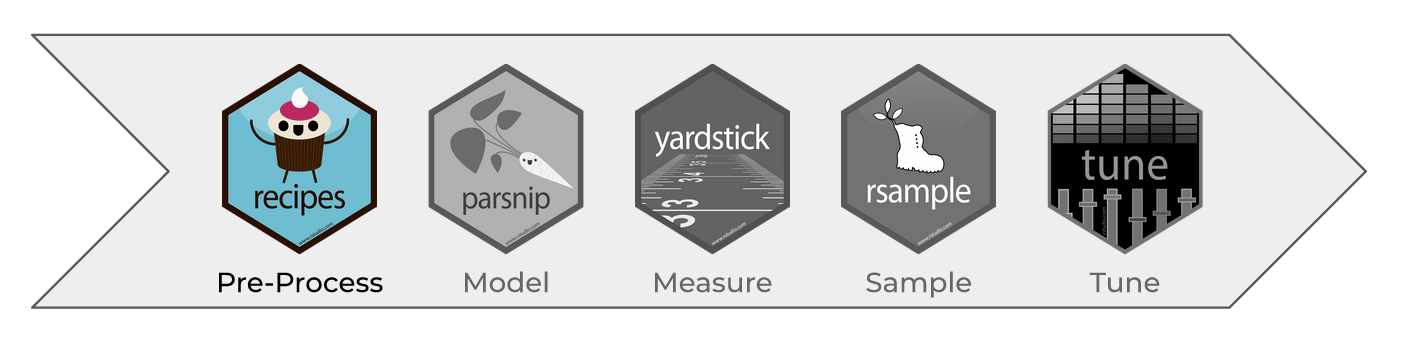
\includegraphics[width=800pt,height=200pt]{img/04-ml/3-2-1-preprocesamiento} \end{center}

Como punto de partida para nuestro flujo de trabajo de aprendizaje automático, necesitaremos datos de entrada.
En la mayoría de los casos, estos datos se cargarán y almacenarán en forma de \emph{data frames} o \emph{tibbles} en R.
Incluirán una o varias variables predictoras y, en caso de aprendizaje supervisado, también incluirán un resultado conocido.

Sin embargo, no todos los modelos pueden lidiar con diferentes problemas de datos y, a menudo,
necesitamos transformar los datos para obtener el mejor rendimiento posible del modelo.
Este proceso se denomina pre-procesamiento y puede incluir una amplia gama de pasos, como:

\begin{itemize}
\tightlist
\item
  \textbf{Dicotomización de variables:} Variables cualitativas que solo pueden tomar
  el valor \(0\) o \(1\) para indicar la ausencia o presencia de una condición específica.
  Estas variables se utilizan para clasificar los datos en categorías mutuamente excluyentes o para activar comandos de encendido / apagado
\end{itemize}

\begin{center}
\includegraphics[width=600pt,height=200pt]{img/04-ml/hombre-mujer} \end{center}

\begin{center}
\includegraphics[width=600pt,height=200pt]{img/04-ml/sino} \end{center}

\begin{itemize}
\tightlist
\item
  \textbf{Near Zero Value (nzv) o Varianza Cero:} En algunas situaciones, el mecanismo de generación de datos puede crear predictores que solo tienen un valor único (es decir, un ``predictor de varianza cercando a cero''). Para muchos modelos (excluidos los modelos basados en árboles), esto puede hacer que el modelo se bloquee o que el ajuste sea inestable.
\end{itemize}

De manera similar, los predictores pueden tener solo una pequeña cantidad de valores únicos que ocurren con frecuencias muy bajas.

\begin{center}
\includegraphics[width=500pt]{img/04-ml/hombres} \end{center}

\begin{itemize}
\tightlist
\item
  \textbf{Imputaciones:} Si faltan algunos predictores, ¿deberían estimarse mediante imputación?
\end{itemize}

\begin{center}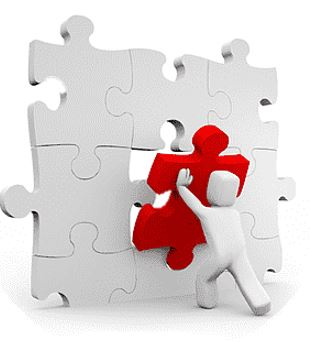
\includegraphics[width=400pt]{img/04-ml/imputar} \end{center}

\begin{itemize}
\tightlist
\item
  \textbf{Des-correlacionar:} Si hay predictores correlacionados, ¿debería mitigarse esta correlación? Esto podría significar filtrar predictores, usar análisis de componentes principales o una técnica basada en modelos (por ejemplo, regularización).
\end{itemize}

\begin{center}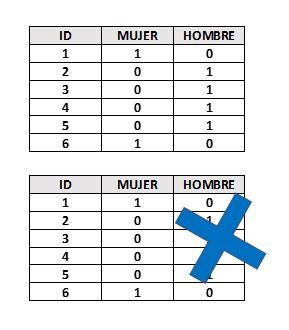
\includegraphics[width=400pt]{img/04-ml/descorrelaciones} \end{center}

\begin{itemize}
\tightlist
\item
  \textbf{Normalizar:} ¿Deben centrarse y escalar los predictores?
\end{itemize}

\begin{center}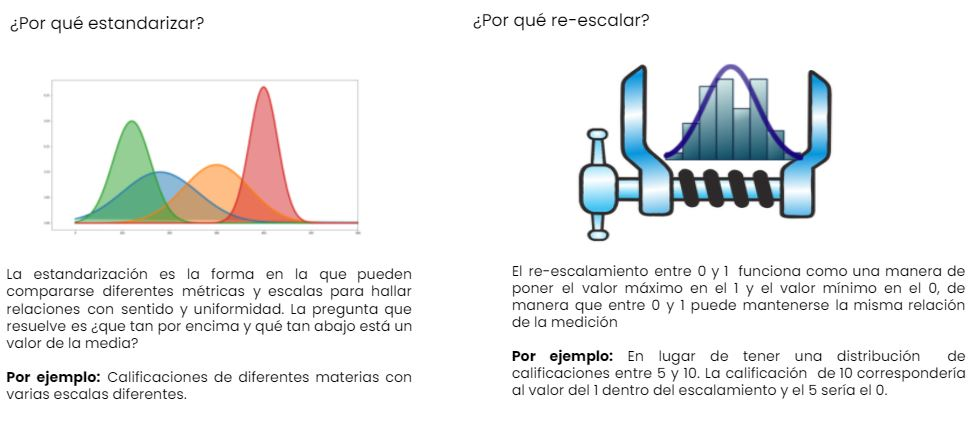
\includegraphics[width=800pt]{img/04-ml/estandarizar-reescalar} \end{center}

\begin{itemize}
\tightlist
\item
  \textbf{Transformar:} ¿Es útil transformar los predictores para que sean más simétricos? (por ejemplo, escala logarítmica).
\end{itemize}

Dependiendo del caso de uso, algunos pasos de pre-procesamiento pueden ser indispensables para pasos posteriores, mientras que otros solo son opcionales. Sin embargo, dependiendo de los pasos de pre-procesamiento elegidos, el rendimiento del modelo puede cambiar significativamente en pasos posteriores. Por lo tanto, es muy común probar varias configuraciones.

En la tabla, \(\checkmark\) indica que el método es obligatorio para el modelo y \(\times\) indica que no lo es. El símbolo \(\circ\) significa que la técnica puede ayudar al modelo, pero no es obligatorio.

\begin{center}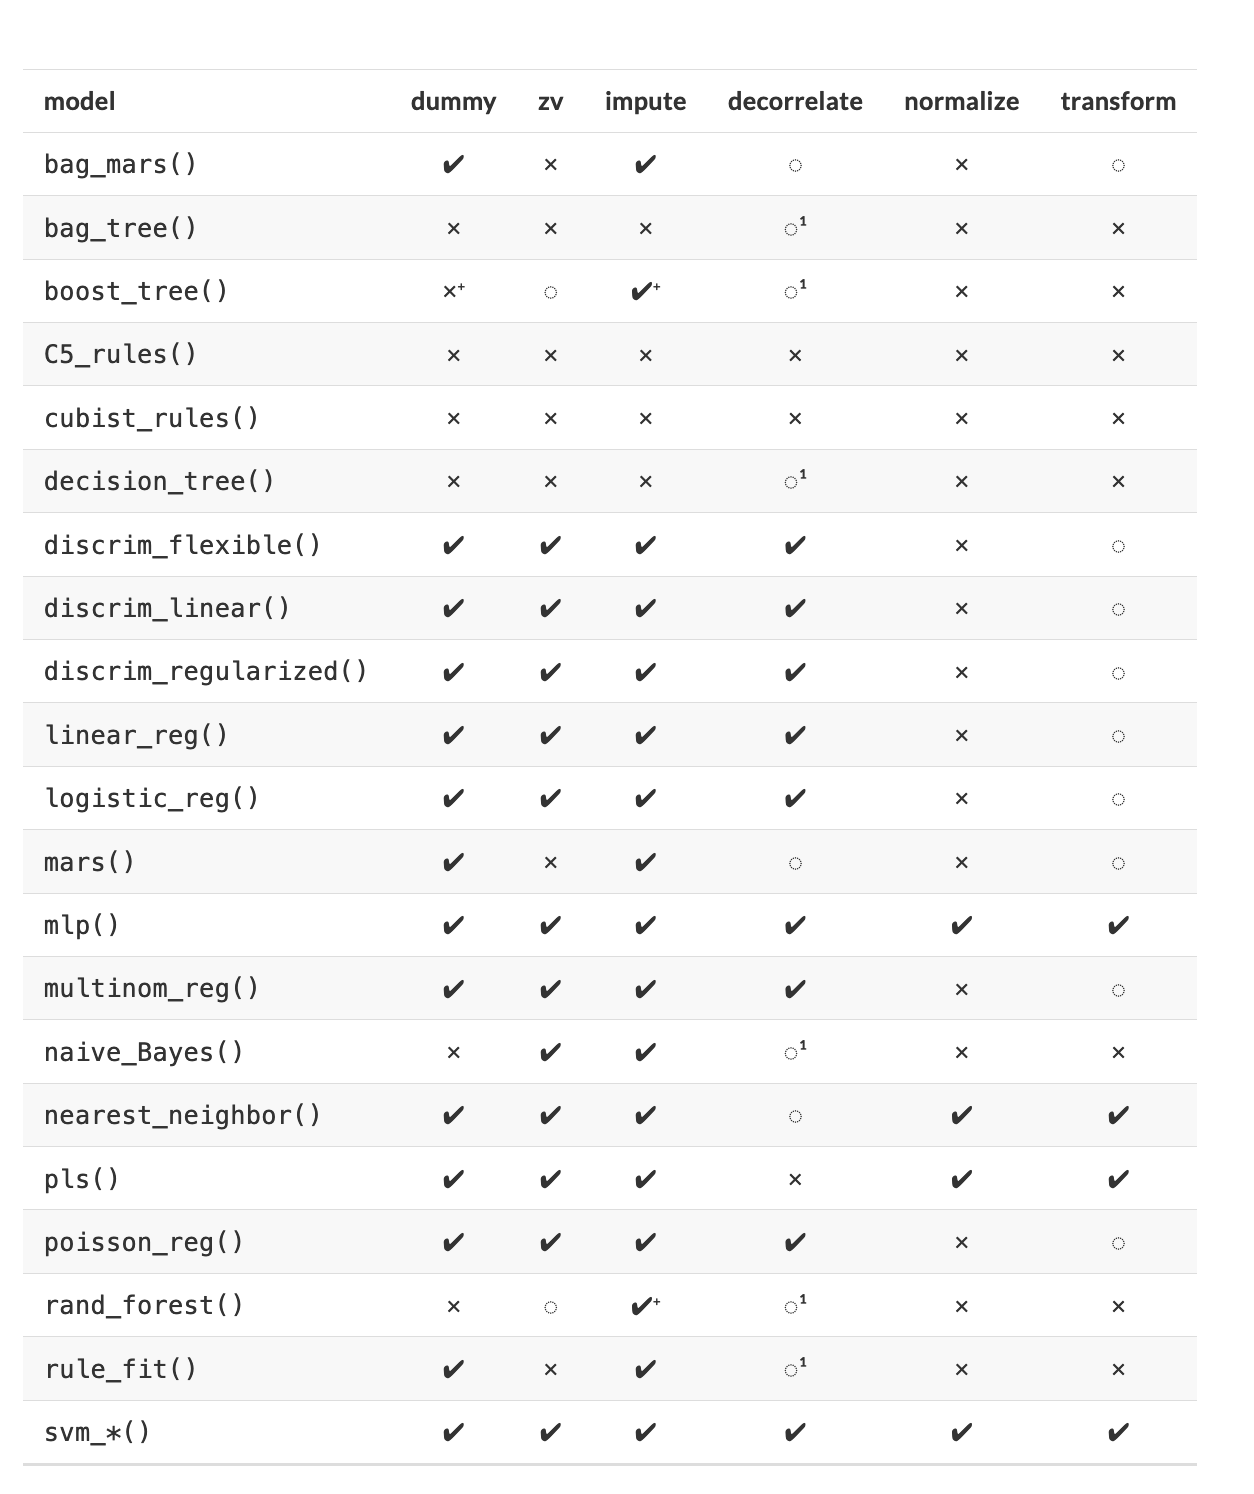
\includegraphics[width=600pt,height=650pt]{img/04-ml/3-2-1-preprocesamiento-modelos} \end{center}

Notación:

\begin{enumerate}
\def\labelenumi{\arabic{enumi}.}
\tightlist
\item
  Es posible que la des-correlación de predictores no ayude a mejorar el rendimiento. Sin embargo, menos predictores correlacionados pueden mejorar la estimación de las puntuaciones de importancia de la varianza.
  Esencialmente, la selección de predictores altamente correlacionados es casi aleatoria.
\end{enumerate}

La notación \(+\) significa que la respuesta depende de la implementación:

\begin{itemize}
\item
  Teoricamente, cualquier modelo basado en árboles no requiere imputación de datos,
  sin embargo, muchas implementaciones de conjuntos de árboles requieren imputación.
\item
  Si bien los métodos de refuerzo basados en árboles generalmente no requieren la creación de variables ficticias, los modelos que usan \texttt{xgboost} sí lo hacen.
\end{itemize}

\hypertarget{ingenieruxeda-de-datos}{%
\subsection{Ingeniería de datos}\label{ingenieruxeda-de-datos}}

La ingeniería de datos abarca actividades que reformatean los valores de los predictores
para que se puedan utilizar de manera eficaz para nuestro modelo.
Esto incluye transformaciones y codificaciones de los datos para representar mejor sus características importantes.

Por ejemplo:

\begin{quote}
\textbf{1.-} Supongamos que un conjunto de datos tiene dos predictores que se pueden representar de manera más eficaz en nuestro modelo como una proporción, así, tendríamos un nuevo predictor a partir de la proporción de los dos predictores originales.
\end{quote}

\begin{table}
\centering
\begin{tabular}[t]{r|r}
\hline
x & x\_prop\\
\hline
691 & 0.1836789\\
\hline
639 & 0.1698565\\
\hline
969 & 0.2575758\\
\hline
955 & 0.2538543\\
\hline
508 & 0.1350346\\
\hline
\end{tabular}
\end{table}

\begin{quote}
\textbf{2.-} Al elegir cómo codificar nuestros datos en el modelado, podríamos elegir una opción que creemos que está más asociada con el resultado. El formato original de los datos, por ejemplo numérico (edad) versus categórico (grupo).
\end{quote}

\begin{table}
\centering
\begin{tabular}[t]{r|l}
\hline
Edad & Grupo\\
\hline
7 & Niños\\
\hline
78 & Adultos mayores\\
\hline
17 & Adolescentes\\
\hline
25 & Adultos\\
\hline
90 & Adultos mayores\\
\hline
\end{tabular}
\end{table}

La ingeniería y el pre-procesamiento de datos también pueden implicar el reformateo requerido por el modelo. Algunos modelos utilizan métricas de distancia geométrica y, en consecuencia, los predictores numéricos deben centrarse y escalar para que estén todos en las mismas unidades. De lo contrario, los valores de distancia estarían sesgados por la escala de cada columna.

\hypertarget{recetas}{%
\section{Recetas}\label{recetas}}

\begin{flushleft}
\includegraphics[width=150pt,height=150pt]{img/04-ml/3-2-3-recetas} \end{flushleft}

Una receta es una \textbf{serie de pasos o instrucciones para el procesamiento de datos.}
A diferencia del método de fórmula dentro de una función de modelado, \textbf{la receta define los pasos sin ejecutarlos} inmediatamente; es sólo una especificación de lo que se debe hacer. La estructura de una receta sigue los siguientes pasos:

\begin{enumerate}
\def\labelenumi{\arabic{enumi}.}
\item
  Inicialización
\item
  Transformación
\item
  Preparación
\item
  Aplicación
\end{enumerate}

La siguiente sección explica la estructura y flujo de transformaciones:

\begin{Shaded}
\begin{Highlighting}[]
\NormalTok{receta }\OtherTok{\textless{}{-}} \FunctionTok{recipe}\NormalTok{(response }\SpecialCharTok{\textasciitilde{}}\NormalTok{ X1 }\SpecialCharTok{+}\NormalTok{ X2 }\SpecialCharTok{+}\NormalTok{ X3 }\SpecialCharTok{+}\NormalTok{ ... }\SpecialCharTok{+}\NormalTok{ Xn, }\AttributeTok{data =}\NormalTok{ dataset ) }\SpecialCharTok{\%\textgreater{}\%} 
  \FunctionTok{transformation\_1}\NormalTok{(...) }\SpecialCharTok{\%\textgreater{}\%} 
  \FunctionTok{transformation\_2}\NormalTok{(...) }\SpecialCharTok{\%\textgreater{}\%} 
  \FunctionTok{transformation\_3}\NormalTok{(...) }\SpecialCharTok{\%\textgreater{}\%} 
\NormalTok{  ...}
  \FunctionTok{final\_transformation}\NormalTok{(...) }\SpecialCharTok{\%\textgreater{}\%} 
  \FunctionTok{prep}\NormalTok{()}

\FunctionTok{bake}\NormalTok{(receta, }\AttributeTok{new\_data =}\NormalTok{ new\_dataset)}
\end{Highlighting}
\end{Shaded}

A continuación se muestran distintos ejemplos de transformaciones realizadas comunmente en el pre-procesamiento de modelos predictivos. Como ejemplo, utilizaremos el subconjunto de predictores disponibles en los datos de vivienda: \texttt{Ames}

\begin{itemize}
\item
  Vecindario (29 vecindarios)
\item
  Superficie habitable bruta sobre el nivel del suelo
\item
  Año de constricción
\item
  Tipo de edificio
\end{itemize}

\textbf{ANTERIORMENTE\ldots{}} Un modelo de regresión lineal ordinario se ajustaba a los datos con la función estándar \texttt{lm()} de la siguiente manera:

\begin{Shaded}
\begin{Highlighting}[]
\FunctionTok{lm}\NormalTok{(Sale\_Price }\SpecialCharTok{\textasciitilde{}}\NormalTok{ Neighborhood }\SpecialCharTok{+} \FunctionTok{log10}\NormalTok{(Gr\_Liv\_Area) }\SpecialCharTok{+}\NormalTok{ Year\_Built }\SpecialCharTok{+}\NormalTok{ Bldg\_Type, }\AttributeTok{data =}\NormalTok{ ames)}
\end{Highlighting}
\end{Shaded}

Cuando se ejecuta esta función, los datos se convierten en a una matriz de diseño numérico (también llamada matriz de modelo) y luego se utiliza el método de mínimos cuadrados para estimar los parámetros.
Lo que hace \textbf{la fórmula anterior se puede descomponer en una serie de pasos:}

\begin{quote}
\textbf{1.-} El precio de venta se define como el resultado, mientras que las variables de vecindario, superficie habitable bruta, año de construcción y tipo de edificio se definen como predictores.
\end{quote}

\begin{quote}
\textbf{2.-} Se aplica una transformación logarítmica al predictor de superficie habitable bruta.
\end{quote}

\begin{quote}
\textbf{3.-} Las columnas de vecindad y tipo de edificio se convierten de un formato no numérico a un formato numérico (dado que los mínimos cuadrados requieren predictores numéricos).
\end{quote}

La siguiente receta es equivalente a la fórmula anterior:

\begin{Shaded}
\begin{Highlighting}[]
\NormalTok{simple\_ames }\OtherTok{\textless{}{-}} \FunctionTok{recipe}\NormalTok{(}
\NormalTok{  Sale\_Price }\SpecialCharTok{\textasciitilde{}}\NormalTok{ Neighborhood }\SpecialCharTok{+}\NormalTok{ Gr\_Liv\_Area }\SpecialCharTok{+}\NormalTok{ Year\_Built }\SpecialCharTok{+}\NormalTok{ Bldg\_Type,}
  \AttributeTok{data =}\NormalTok{ ames) }\SpecialCharTok{\%\textgreater{}\%}
  \FunctionTok{step\_log}\NormalTok{(Gr\_Liv\_Area, }\AttributeTok{base =} \DecValTok{10}\NormalTok{) }\SpecialCharTok{\%\textgreater{}\%} 
  \FunctionTok{step\_dummy}\NormalTok{(}\FunctionTok{all\_nominal\_predictors}\NormalTok{())}

\NormalTok{simple\_ames}
\end{Highlighting}
\end{Shaded}

\begin{verbatim}
## Recipe
## 
## Inputs:
## 
##       role #variables
##    outcome          1
##  predictor          4
## 
## Operations:
## 
## Log transformation on Gr_Liv_Area
## Dummy variables from all_nominal_predictors()
\end{verbatim}

\textbf{Ventajas de usar una receta:}

\begin{itemize}
\item
  \textbf{Los cálculos se pueden reciclar entre modelos} ya que no están estrechamente acoplados a la función de modelado.
\item
  Una receta permite un \textbf{conjunto más amplio de opciones de procesamiento} de datos que las que pueden ofrecer las fórmulas.
\item
  La \textbf{sintaxis puede ser muy compacta}. Por ejemplo, \texttt{all\_nominal\_predictors()} se puede usar para capturar muchas variables para tipos específicos de procesamiento, mientras que una fórmula requeriría que cada una se enumere explícitamente.
\item
  Todo el procesamiento de datos se puede capturar en un solo objeto en lugar de tener scripts que se repiten o incluso se distribuyen en diferentes archivos.
\end{itemize}

\hypertarget{pasos-y-estructura-de-recetas}{%
\subsection{Pasos y estructura de recetas}\label{pasos-y-estructura-de-recetas}}

Como se mostró anteriormente, existen 4 pasos fundamentales para el procesamiento y transformación de conjuntos de datos. Estos pasos se describen de la siguiente manera:

\begin{itemize}
\item
  \textbf{Receta:} Inicializa una receta y define los roles de las variables
\item
  \textbf{Transformaciones:} Mutaciones a los renglones y columnas hasta desear el resultado
\item
  \textbf{Preparación:} Se realizan las estimaciones estadísticas con los datos
\end{itemize}

La función \textbf{\texttt{prep()}} estima las cantidades requeridas y las estadísticas necesarias para cualquier paso declarado en la receta.

\begin{Shaded}
\begin{Highlighting}[]
\NormalTok{prep }\OtherTok{\textless{}{-}} \FunctionTok{prep}\NormalTok{(simple\_ames) }

\NormalTok{prep}
\end{Highlighting}
\end{Shaded}

\begin{verbatim}
## Recipe
## 
## Inputs:
## 
##       role #variables
##    outcome          1
##  predictor          4
## 
## Training data contained 2930 data points and no missing data.
## 
## Operations:
## 
## Log transformation on Gr_Liv_Area [trained]
## Dummy variables from Neighborhood, Bldg_Type [trained]
\end{verbatim}

\begin{itemize}
\tightlist
\item
  \textbf{Aplicación} Se llevan a cabo las transformaciones especificadas en la receta preparada a un conjunto de datos.
\end{itemize}

Finalmente, la función \textbf{\texttt{bake()}} lleva a cabo la transformación de un conjunto de datos a través de las estimaciones indicadas en una receta y \textbf{aplica las operaciones a un conjunto de datos para crear una matriz de diseño}. La función \texttt{bake(object,\ new\_data\ =\ NULL)} devolverá los datos con los que se entrenó la receta.

\textbf{Nota: } La función \textbf{\texttt{juice()}} devolverá los resultados de una receta en la que se hayan aplicado todos los pasos a los datos. Similar a la función \texttt{bake()} con el comando \texttt{new\_data\ =\ NULL}.

\begin{Shaded}
\begin{Highlighting}[]
\NormalTok{simple\_ames }\SpecialCharTok{\%\textgreater{}\%} 
  \FunctionTok{prep}\NormalTok{() }\SpecialCharTok{\%\textgreater{}\%} 
  \FunctionTok{bake}\NormalTok{(}\AttributeTok{new\_data =} \ConstantTok{NULL}\NormalTok{) }\SpecialCharTok{\%\textgreater{}\%} 
  \FunctionTok{glimpse}\NormalTok{()}
\end{Highlighting}
\end{Shaded}

\begin{verbatim}
## Rows: 2,930
## Columns: 35
## $ Gr_Liv_Area                                          <dbl> 3.219060, 2.95230~
## $ Year_Built                                           <int> 1960, 1961, 1958,~
## $ Sale_Price                                           <int> 215000, 105000, 1~
## $ Neighborhood_College_Creek                           <dbl> 0, 0, 0, 0, 0, 0,~
## $ Neighborhood_Old_Town                                <dbl> 0, 0, 0, 0, 0, 0,~
## $ Neighborhood_Edwards                                 <dbl> 0, 0, 0, 0, 0, 0,~
## $ Neighborhood_Somerset                                <dbl> 0, 0, 0, 0, 0, 0,~
## $ Neighborhood_Northridge_Heights                      <dbl> 0, 0, 0, 0, 0, 0,~
## $ Neighborhood_Gilbert                                 <dbl> 0, 0, 0, 0, 1, 1,~
## $ Neighborhood_Sawyer                                  <dbl> 0, 0, 0, 0, 0, 0,~
## $ Neighborhood_Northwest_Ames                          <dbl> 0, 0, 0, 0, 0, 0,~
## $ Neighborhood_Sawyer_West                             <dbl> 0, 0, 0, 0, 0, 0,~
## $ Neighborhood_Mitchell                                <dbl> 0, 0, 0, 0, 0, 0,~
## $ Neighborhood_Brookside                               <dbl> 0, 0, 0, 0, 0, 0,~
## $ Neighborhood_Crawford                                <dbl> 0, 0, 0, 0, 0, 0,~
## $ Neighborhood_Iowa_DOT_and_Rail_Road                  <dbl> 0, 0, 0, 0, 0, 0,~
## $ Neighborhood_Timberland                              <dbl> 0, 0, 0, 0, 0, 0,~
## $ Neighborhood_Northridge                              <dbl> 0, 0, 0, 0, 0, 0,~
## $ Neighborhood_Stone_Brook                             <dbl> 0, 0, 0, 0, 0, 0,~
## $ Neighborhood_South_and_West_of_Iowa_State_University <dbl> 0, 0, 0, 0, 0, 0,~
## $ Neighborhood_Clear_Creek                             <dbl> 0, 0, 0, 0, 0, 0,~
## $ Neighborhood_Meadow_Village                          <dbl> 0, 0, 0, 0, 0, 0,~
## $ Neighborhood_Briardale                               <dbl> 0, 0, 0, 0, 0, 0,~
## $ Neighborhood_Bloomington_Heights                     <dbl> 0, 0, 0, 0, 0, 0,~
## $ Neighborhood_Veenker                                 <dbl> 0, 0, 0, 0, 0, 0,~
## $ Neighborhood_Northpark_Villa                         <dbl> 0, 0, 0, 0, 0, 0,~
## $ Neighborhood_Blueste                                 <dbl> 0, 0, 0, 0, 0, 0,~
## $ Neighborhood_Greens                                  <dbl> 0, 0, 0, 0, 0, 0,~
## $ Neighborhood_Green_Hills                             <dbl> 0, 0, 0, 0, 0, 0,~
## $ Neighborhood_Landmark                                <dbl> 0, 0, 0, 0, 0, 0,~
## $ Neighborhood_Hayden_Lake                             <dbl> 0, 0, 0, 0, 0, 0,~
## $ Bldg_Type_TwoFmCon                                   <dbl> 0, 0, 0, 0, 0, 0,~
## $ Bldg_Type_Duplex                                     <dbl> 0, 0, 0, 0, 0, 0,~
## $ Bldg_Type_Twnhs                                      <dbl> 0, 0, 0, 0, 0, 0,~
## $ Bldg_Type_TwnhsE                                     <dbl> 0, 0, 0, 0, 0, 0,~
\end{verbatim}

En cuanto a las transformaciones posibles, existe una gran cantidad de funciones que soportan este proceso. En esta sección se muestran algunas de las transformación más comunes, entre ellas:

\begin{itemize}
\tightlist
\item
  Normalización
\item
  Dicotomización
\item
  Creación de nuevas columnas
\item
  Datos faltantes
\item
  Imputaciones
\item
  Interacciones
\item
  Etc.
\end{itemize}

\hypertarget{normalizar-columnas-numuxe9ricas}{%
\subsubsection{Normalizar columnas numéricas}\label{normalizar-columnas-numuxe9ricas}}

Quizá la transformación numérica más usada en todos los modelos es la estandarización o normalización de variables numéricas. \textbf{Este proceso se realiza para homologar la escala de las variables numéricas}, de modo que no predomine una sobre otra debido a la diferencia de magnitudes o escalas. Este proceso se tiene de fondo el siguiente proceso estadístico:

\[Z=\frac{X-\hat{\mu}_x}{\hat{\sigma}_x}\]

\textbf{Donde:}

\begin{itemize}
\item
  X = Es una variable o columna numérica
\item
  \(\hat{\mu}_x\) = Es la estimación de la media de la variable \emph{X}
\item
  \(\hat{\sigma}_x\) = Es la estimación de la desviación estándar de la variable \emph{X}
\end{itemize}

La librería recipes nos permite realizar este proceso ágilmente mediante la función: \texttt{step\_normalize()}.

\begin{Shaded}
\begin{Highlighting}[]
\NormalTok{ames }\SpecialCharTok{\%\textgreater{}\%} \FunctionTok{select}\NormalTok{(Sale\_Price, Neighborhood, Gr\_Liv\_Area, Year\_Built, Bldg\_Type) }\SpecialCharTok{\%\textgreater{}\%} 
  \FunctionTok{head}\NormalTok{(}\DecValTok{5}\NormalTok{)}
\end{Highlighting}
\end{Shaded}

\begin{verbatim}
## # A tibble: 5 x 5
##   Sale_Price Neighborhood Gr_Liv_Area Year_Built Bldg_Type
##        <int> <fct>              <int>      <int> <fct>    
## 1     215000 North_Ames          1656       1960 OneFam   
## 2     105000 North_Ames           896       1961 OneFam   
## 3     172000 North_Ames          1329       1958 OneFam   
## 4     244000 North_Ames          2110       1968 OneFam   
## 5     189900 Gilbert             1629       1997 OneFam
\end{verbatim}

\begin{Shaded}
\begin{Highlighting}[]
\NormalTok{simple\_ames }\OtherTok{\textless{}{-}} \FunctionTok{recipe}\NormalTok{(Sale\_Price }\SpecialCharTok{\textasciitilde{}}\NormalTok{ ., }\AttributeTok{data =}\NormalTok{ ames) }\SpecialCharTok{\%\textgreater{}\%}
  \FunctionTok{step\_normalize}\NormalTok{(}\FunctionTok{all\_numeric\_predictors}\NormalTok{())}

\NormalTok{simple\_ames}
\end{Highlighting}
\end{Shaded}

\begin{verbatim}
## Recipe
## 
## Inputs:
## 
##       role #variables
##    outcome          1
##  predictor         73
## 
## Operations:
## 
## Centering and scaling for all_numeric_predictors()
\end{verbatim}

\begin{Shaded}
\begin{Highlighting}[]
\NormalTok{simple\_ames }\SpecialCharTok{\%\textgreater{}\%} 
  \FunctionTok{prep}\NormalTok{() }\SpecialCharTok{\%\textgreater{}\%} 
  \FunctionTok{bake}\NormalTok{(}\AttributeTok{new\_data =} \ConstantTok{NULL}\NormalTok{) }\SpecialCharTok{\%\textgreater{}\%} 
  \FunctionTok{select}\NormalTok{(Sale\_Price, Neighborhood, Gr\_Liv\_Area, Year\_Built, Bldg\_Type) }\SpecialCharTok{\%\textgreater{}\%} 
  \FunctionTok{head}\NormalTok{(}\DecValTok{5}\NormalTok{)}
\end{Highlighting}
\end{Shaded}

\begin{verbatim}
## # A tibble: 5 x 5
##   Sale_Price Neighborhood Gr_Liv_Area Year_Built Bldg_Type
##        <int> <fct>              <dbl>      <dbl> <fct>    
## 1     215000 North_Ames         0.309     -0.375 OneFam   
## 2     105000 North_Ames        -1.19      -0.342 OneFam   
## 3     172000 North_Ames        -0.338     -0.442 OneFam   
## 4     244000 North_Ames         1.21      -0.111 OneFam   
## 5     189900 Gilbert            0.256      0.848 OneFam
\end{verbatim}

\hypertarget{dicotomizaciuxf3n-de-categoruxedas}{%
\subsubsection{Dicotomización de categorías}\label{dicotomizaciuxf3n-de-categoruxedas}}

Otra transformación necesaria en la mayoría de los modelos predictivos en la creación de las variables dummy. Se mencionó anteriormente que los modelos requieren de una matriz numérica de características explicativas que permita calcular patrones estadísticos para predecir la variable de respuesta. El proceso de dicotomización consiste en \textbf{crear una variable dicotómica por cada categoría de una columna con valores nominales}.

\begin{Shaded}
\begin{Highlighting}[]
\NormalTok{ames }\SpecialCharTok{\%\textgreater{}\%} \FunctionTok{select}\NormalTok{(Sale\_Price, Bldg\_Type) }\SpecialCharTok{\%\textgreater{}\%} \FunctionTok{head}\NormalTok{(}\DecValTok{5}\NormalTok{)}
\end{Highlighting}
\end{Shaded}

\begin{verbatim}
## # A tibble: 5 x 2
##   Sale_Price Bldg_Type
##        <int> <fct>    
## 1     215000 OneFam   
## 2     105000 OneFam   
## 3     172000 OneFam   
## 4     244000 OneFam   
## 5     189900 OneFam
\end{verbatim}

\begin{Shaded}
\begin{Highlighting}[]
\NormalTok{ames }\SpecialCharTok{\%\textgreater{}\%} \FunctionTok{select}\NormalTok{(Bldg\_Type) }\SpecialCharTok{\%\textgreater{}\%} \FunctionTok{distinct}\NormalTok{() }\SpecialCharTok{\%\textgreater{}\%} \FunctionTok{pull}\NormalTok{()}
\end{Highlighting}
\end{Shaded}

\begin{verbatim}
## [1] OneFam   TwnhsE   Twnhs    Duplex   TwoFmCon
## Levels: OneFam TwoFmCon Duplex Twnhs TwnhsE
\end{verbatim}

\begin{Shaded}
\begin{Highlighting}[]
\NormalTok{simple\_ames }\OtherTok{\textless{}{-}} \FunctionTok{recipe}\NormalTok{(Sale\_Price }\SpecialCharTok{\textasciitilde{}}\NormalTok{ Bldg\_Type, }\AttributeTok{data =}\NormalTok{ ames) }\SpecialCharTok{\%\textgreater{}\%}
  \FunctionTok{step\_dummy}\NormalTok{(}\FunctionTok{all\_nominal\_predictors}\NormalTok{()) }\SpecialCharTok{\%\textgreater{}\%} 
  \FunctionTok{prep}\NormalTok{()}

\NormalTok{simple\_ames}
\end{Highlighting}
\end{Shaded}

\begin{verbatim}
## Recipe
## 
## Inputs:
## 
##       role #variables
##    outcome          1
##  predictor          1
## 
## Training data contained 2930 data points and no missing data.
## 
## Operations:
## 
## Dummy variables from Bldg_Type [trained]
\end{verbatim}

\begin{Shaded}
\begin{Highlighting}[]
\NormalTok{simple\_ames }\SpecialCharTok{\%\textgreater{}\%} \FunctionTok{bake}\NormalTok{(}\AttributeTok{new\_data =} \ConstantTok{NULL}\NormalTok{) }\SpecialCharTok{\%\textgreater{}\%} \FunctionTok{head}\NormalTok{(}\DecValTok{5}\NormalTok{)}
\end{Highlighting}
\end{Shaded}

\begin{verbatim}
## # A tibble: 5 x 5
##   Sale_Price Bldg_Type_TwoFmC~ Bldg_Type_Duplex Bldg_Type_Twnhs Bldg_Type_TwnhsE
##        <int>             <dbl>            <dbl>           <dbl>            <dbl>
## 1     215000                 0                0               0                0
## 2     105000                 0                0               0                0
## 3     172000                 0                0               0                0
## 4     244000                 0                0               0                0
## 5     189900                 0                0               0                0
\end{verbatim}

El proceso de dicotomización demanda que únicamente \texttt{(n-1)} categorías sean expresadas, mientras que la restante será considerada la \textbf{categoría default o basal}. Esta última categoría es la usada en el modelo cuando todas las demás se encuentran ausentes.

\hypertarget{codificaciuxf3n-de-datos-cualitativos-nuevos-o-faltantes}{%
\subsubsection{Codificación de datos cualitativos nuevos o faltantes}\label{codificaciuxf3n-de-datos-cualitativos-nuevos-o-faltantes}}

Una de las tareas de ingeniería de datos más comunes es el tratamiento de datos faltantes, datos no antes vistos y datos con poca frecuencia. \textbf{El problema principal con estos casos es que los modelos no saben cómo relacionar estos eventos con futuras predicciones}. Es conveniente realizar las transformaciones necesarias de tratamiento de estos datos antes de pasar a la etapa de modelado.

Por ejemplo:

\begin{itemize}
\item
  \texttt{step\_unknown()} cambia los valores perdidos en un nivel de factor ``desconocido''.
\item
  \texttt{step\_other()} analiza las frecuencias de los niveles de los factores en el conjunto de datos y convierte los valores que ocurren con poca frecuencia a un nivel general de ``otro'', con un umbral que se puede especificar.
\item
  \texttt{step\_novel()} puede asignar un nuevo nivel si anticipamos que se puede encontrar un nuevo factor en datos futuros.
\end{itemize}

Un buen ejemplo es el predictor de \textbf{vecindad} en nuestros datos. Aquí hay dos vecindarios que tienen menos de cinco propiedades.

\begin{Shaded}
\begin{Highlighting}[]
\FunctionTok{ggplot}\NormalTok{(}\AttributeTok{data =}\NormalTok{ ames, }\FunctionTok{aes}\NormalTok{(}\AttributeTok{y =}\NormalTok{ Neighborhood)) }\SpecialCharTok{+} 
  \FunctionTok{geom\_bar}\NormalTok{() }\SpecialCharTok{+} 
  \FunctionTok{labs}\NormalTok{(}\AttributeTok{y =} \ConstantTok{NULL}\NormalTok{)}
\end{Highlighting}
\end{Shaded}

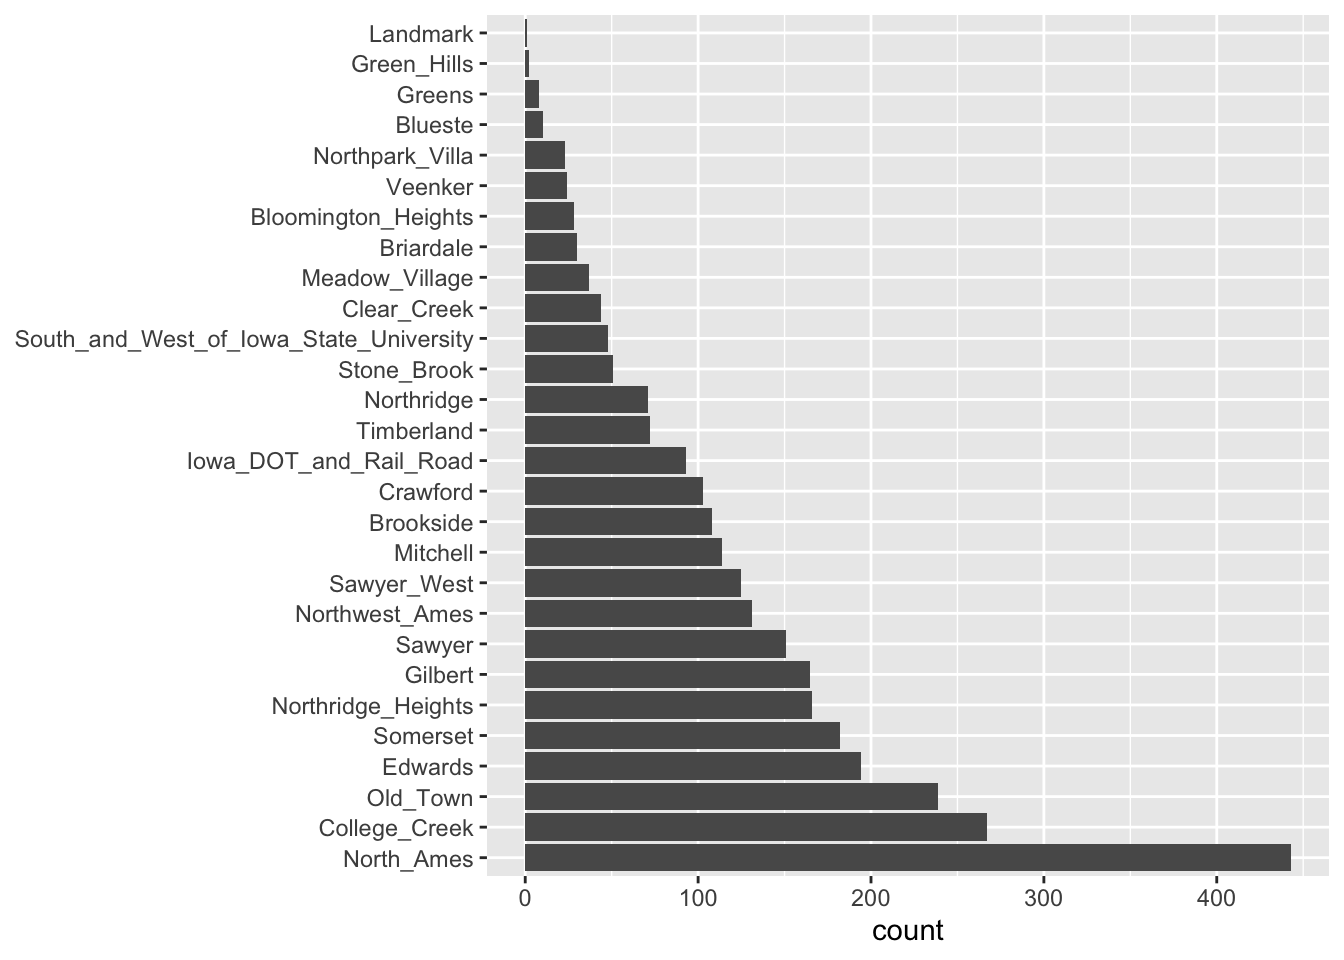
\includegraphics{amt22_03intro2mls2_files/figure-latex/unnamed-chunk-29-1.pdf}

Para algunos modelos, puede resultar problemático tener variables dummy con una sola entrada distinta de cero en la columna. Como mínimo, es muy improbable que estas características sean importantes para un modelo.

Si agregamos \texttt{step\_other\ (Neighborhood,\ threshold\ =\ 0.01)} a nuestra receta, el último \(1\%\) de los vecindarios se agrupará en un nuevo nivel llamado ``otro'', esto atrapará a 8 vecindarios.

\begin{Shaded}
\begin{Highlighting}[]
\NormalTok{simple\_ames }\OtherTok{\textless{}{-}} \FunctionTok{recipe}\NormalTok{(}
\NormalTok{  Sale\_Price }\SpecialCharTok{\textasciitilde{}}\NormalTok{ Neighborhood }\SpecialCharTok{+}\NormalTok{ Gr\_Liv\_Area }\SpecialCharTok{+}\NormalTok{ Year\_Built }\SpecialCharTok{+}\NormalTok{ Bldg\_Type,}
  \AttributeTok{data =}\NormalTok{ ames) }\SpecialCharTok{\%\textgreater{}\%}
  \FunctionTok{step\_other}\NormalTok{(Neighborhood, }\AttributeTok{threshold =} \FloatTok{0.01}\NormalTok{) }\SpecialCharTok{\%\textgreater{}\%} 
  \FunctionTok{prep}\NormalTok{()}

\NormalTok{ejemplo }\OtherTok{\textless{}{-}} \FunctionTok{juice}\NormalTok{(simple\_ames)}

\FunctionTok{ggplot}\NormalTok{(ejemplo, }\FunctionTok{aes}\NormalTok{(}\AttributeTok{y =}\NormalTok{ Neighborhood)) }\SpecialCharTok{+} 
  \FunctionTok{geom\_bar}\NormalTok{() }\SpecialCharTok{+} 
  \FunctionTok{labs}\NormalTok{(}\AttributeTok{y =} \ConstantTok{NULL}\NormalTok{)}
\end{Highlighting}
\end{Shaded}

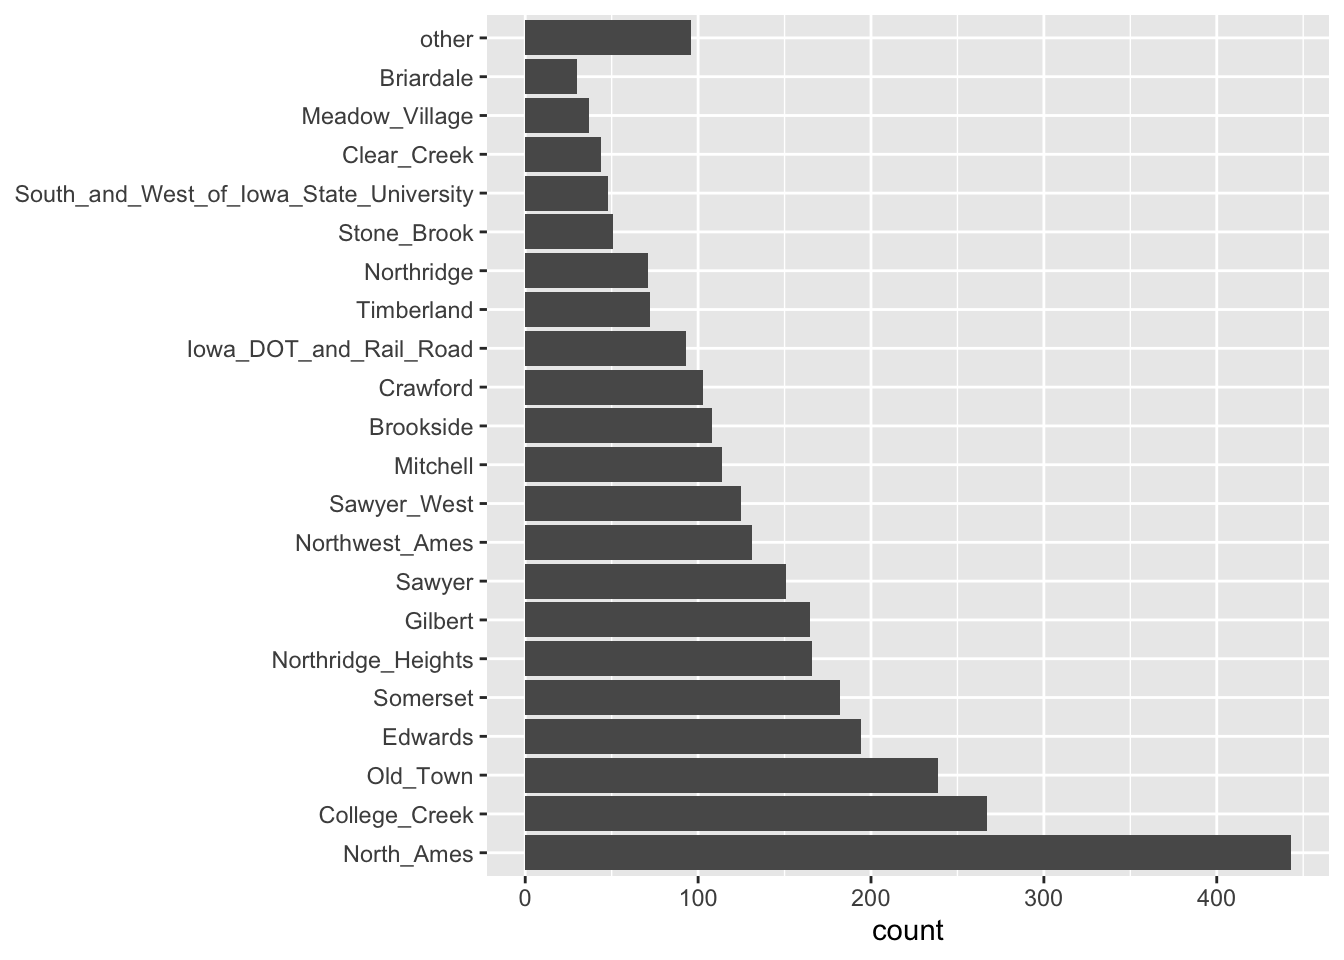
\includegraphics{amt22_03intro2mls2_files/figure-latex/unnamed-chunk-30-1.pdf}

\hypertarget{imputaciones}{%
\subsection{Imputaciones}\label{imputaciones}}

La función \texttt{step\_unknown} crea una categoría nombrada \texttt{unknown}, la cual sirve como reemplazo de datos categóricos faltantes, sin embargo, para imputar datos numéricos se requiere de otra estrategia. Las imputaciones o sustituciones más comunes son realizadas a través de medidas de tendencia central tales como la media y mediana. A continuación se muestra un ejemplo:

\begin{Shaded}
\begin{Highlighting}[]
\NormalTok{ames\_na }\OtherTok{\textless{}{-}}\NormalTok{ ames}
\NormalTok{ames\_na[}\FunctionTok{sample}\NormalTok{(}\FunctionTok{nrow}\NormalTok{(ames), }\DecValTok{5}\NormalTok{), }\FunctionTok{c}\NormalTok{(}\StringTok{"Gr\_Liv\_Area"}\NormalTok{, }\StringTok{"Lot\_Area"}\NormalTok{)] }\OtherTok{\textless{}{-}} \ConstantTok{NA}

\NormalTok{ames\_na }\SpecialCharTok{\%\textgreater{}\%} \FunctionTok{filter}\NormalTok{(}\FunctionTok{is.na}\NormalTok{(Gr\_Liv\_Area) }\SpecialCharTok{|} \FunctionTok{is.na}\NormalTok{(Lot\_Area)) }\SpecialCharTok{\%\textgreater{}\%} 
  \FunctionTok{select}\NormalTok{(Sale\_Price, Gr\_Liv\_Area, Lot\_Area)}
\end{Highlighting}
\end{Shaded}

\begin{verbatim}
## # A tibble: 5 x 3
##   Sale_Price Gr_Liv_Area Lot_Area
##        <int>       <int>    <int>
## 1     153000          NA       NA
## 2     180000          NA       NA
## 3     170000          NA       NA
## 4     215000          NA       NA
## 5     157000          NA       NA
\end{verbatim}

\begin{Shaded}
\begin{Highlighting}[]
\NormalTok{simple\_ames }\OtherTok{\textless{}{-}} \FunctionTok{recipe}\NormalTok{(Sale\_Price }\SpecialCharTok{\textasciitilde{}}\NormalTok{ Gr\_Liv\_Area }\SpecialCharTok{+}\NormalTok{ Lot\_Area, }\AttributeTok{data =}\NormalTok{ ames\_na) }\SpecialCharTok{\%\textgreater{}\%}
  \FunctionTok{step\_impute\_mean}\NormalTok{(Gr\_Liv\_Area) }\SpecialCharTok{\%\textgreater{}\%} 
  \FunctionTok{step\_impute\_median}\NormalTok{(Lot\_Area) }\SpecialCharTok{\%\textgreater{}\%} 
  \FunctionTok{prep}\NormalTok{()}

\FunctionTok{bake}\NormalTok{(simple\_ames, }\AttributeTok{new\_data =}\NormalTok{ ames\_na) }\SpecialCharTok{\%\textgreater{}\%} 
  \FunctionTok{filter}\NormalTok{(}\FunctionTok{is.na}\NormalTok{(Gr\_Liv\_Area) }\SpecialCharTok{|} \FunctionTok{is.na}\NormalTok{(Lot\_Area))}
\end{Highlighting}
\end{Shaded}

\begin{verbatim}
## # A tibble: 0 x 3
## # ... with 3 variables: Gr_Liv_Area <int>, Lot_Area <int>, Sale_Price <int>
\end{verbatim}

Forzamos algunos renglones a que sean omitidos aleatoriamente. Posteriormente, estos valores son imputados mediante su media y mediana.

\hypertarget{agregar-o-modificar-columnas}{%
\subsection{Agregar o modificar columnas}\label{agregar-o-modificar-columnas}}

Quizá la transformación más usada sea la agregación o mutación de columnas existentes. Similar a la función \texttt{mutate()} de \emph{dplyr}, la función \texttt{step\_mutate()} se encarga de realizar esta tarea dentro de un pipeline o receta.

\begin{Shaded}
\begin{Highlighting}[]
\NormalTok{ejemplo }\OtherTok{\textless{}{-}} \FunctionTok{recipe}\NormalTok{(}
\NormalTok{  Sale\_Price }\SpecialCharTok{\textasciitilde{}}\NormalTok{ Neighborhood }\SpecialCharTok{+}\NormalTok{ Gr\_Liv\_Area }\SpecialCharTok{+}\NormalTok{ Year\_Built }\SpecialCharTok{+}\NormalTok{ Bldg\_Type }\SpecialCharTok{+}\NormalTok{ Year\_Remod\_Add,}
  \AttributeTok{data =}\NormalTok{ ames) }\SpecialCharTok{\%\textgreater{}\%}
  \FunctionTok{step\_mutate}\NormalTok{(}
    \AttributeTok{Sale\_Price\_Peso =}\NormalTok{ Sale\_Price }\SpecialCharTok{*} \FloatTok{19.87}\NormalTok{,}
    \AttributeTok{Last\_Inversion =}\NormalTok{ Year\_Remod\_Add }\SpecialCharTok{{-}}\NormalTok{ Year\_Built}
\NormalTok{    ) }\SpecialCharTok{\%\textgreater{}\%} 
  \FunctionTok{step\_arrange}\NormalTok{(}\FunctionTok{desc}\NormalTok{(Last\_Inversion)) }\SpecialCharTok{\%\textgreater{}\%} 
  \FunctionTok{prep}\NormalTok{()}

\NormalTok{ejemplo}
\end{Highlighting}
\end{Shaded}

\begin{verbatim}
## Recipe
## 
## Inputs:
## 
##       role #variables
##    outcome          1
##  predictor          5
## 
## Training data contained 2930 data points and no missing data.
## 
## Operations:
## 
## Variable mutation for ~Sale_Price * 19.87, ~Year_Remod_Add - Yea... [trained]
## Row arrangement using ~desc(Last_Inversion) [trained]
\end{verbatim}

\begin{Shaded}
\begin{Highlighting}[]
\NormalTok{ejemplo }\SpecialCharTok{\%\textgreater{}\%} \FunctionTok{bake}\NormalTok{(}\AttributeTok{new\_data =} \ConstantTok{NULL}\NormalTok{) }\SpecialCharTok{\%\textgreater{}\%} 
  \FunctionTok{select}\NormalTok{(Sale\_Price, Sale\_Price\_Peso, Year\_Remod\_Add, Year\_Built, Last\_Inversion)}
\end{Highlighting}
\end{Shaded}

\begin{verbatim}
## # A tibble: 2,930 x 5
##    Sale_Price Sale_Price_Peso Year_Remod_Add Year_Built Last_Inversion
##         <int>           <dbl>          <int>      <int>          <int>
##  1     131000        2602970            2007       1880            127
##  2     265979        5285003.           2003       1880            123
##  3     295000        5861650            2002       1880            122
##  4      94000        1867780            1996       1875            121
##  5     138000        2742060            2006       1890            116
##  6     122000        2424140            1987       1872            115
##  7     240000        4768800            2002       1890            112
##  8     119600        2376452            2006       1895            111
##  9     124000        2463880            1991       1880            111
## 10     100000        1987000            1995       1885            110
## # ... with 2,920 more rows
\end{verbatim}

En este ejemplo se realiza la creación de una nueva variable y la modificación de una ya existente.

\hypertarget{interacciones}{%
\subsection{Interacciones}\label{interacciones}}

Los efectos de interacción involucran dos o más predictores. Tal efecto \textbf{ocurre cuando un predictor tiene un efecto sobre el resultado que depende de uno o más predictores.}

Numéricamente, un término de interacción entre predictores se codifica como su producto. Las interacciones solo se definen en términos de su efecto sobre el resultado y pueden ser combinaciones de diferentes tipos de datos (por ejemplo, numéricos, categóricos, etc.).

Después de explorar el conjunto de datos de Ames, podríamos encontrar que las pendientes
de regresión para el área habitable bruta difieren para los diferentes tipos de edificios:

\begin{Shaded}
\begin{Highlighting}[]
\FunctionTok{ggplot}\NormalTok{(ames, }\FunctionTok{aes}\NormalTok{(}\AttributeTok{x =}\NormalTok{ Gr\_Liv\_Area, }\AttributeTok{y =}\NormalTok{ Sale\_Price)) }\SpecialCharTok{+} 
  \FunctionTok{geom\_point}\NormalTok{(}\AttributeTok{alpha =}\NormalTok{ .}\DecValTok{2}\NormalTok{) }\SpecialCharTok{+}
  \FunctionTok{facet\_wrap}\NormalTok{(}\SpecialCharTok{\textasciitilde{}}\NormalTok{ Bldg\_Type) }\SpecialCharTok{+} 
  \FunctionTok{geom\_smooth}\NormalTok{(}\AttributeTok{method =}\NormalTok{ lm, }\AttributeTok{formula =}\NormalTok{ y }\SpecialCharTok{\textasciitilde{}}\NormalTok{ x, }\AttributeTok{se =} \ConstantTok{FALSE}\NormalTok{, }\AttributeTok{col =} \StringTok{"red"}\NormalTok{) }\SpecialCharTok{+} 
  \FunctionTok{scale\_x\_log10}\NormalTok{() }\SpecialCharTok{+} 
  \FunctionTok{scale\_y\_log10}\NormalTok{() }\SpecialCharTok{+} 
  \FunctionTok{labs}\NormalTok{(}\AttributeTok{x =} \StringTok{"Gross Living Area"}\NormalTok{, }\AttributeTok{y =} \StringTok{"Sale Price (USD)"}\NormalTok{)}
\end{Highlighting}
\end{Shaded}

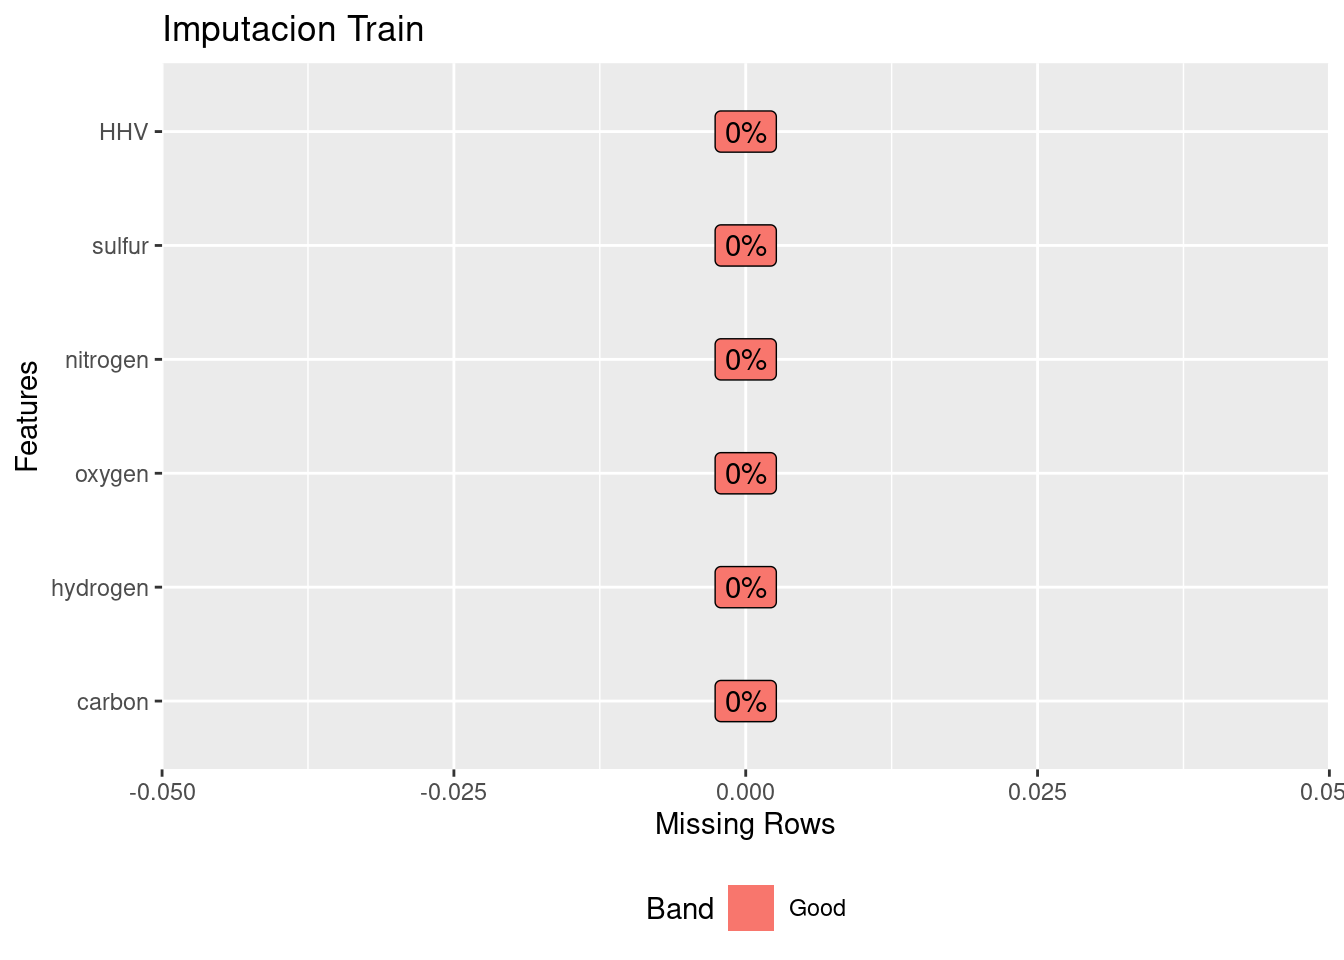
\includegraphics{amt22_03intro2mls2_files/figure-latex/unnamed-chunk-33-1.pdf}

Con la receta actual, \texttt{step\_dummy()} ya ha creado variables ficticias.
¿Cómo combinaríamos estos para una interacción? El paso adicional se vería como
\texttt{step\_interact(\textasciitilde{}\ términos\ de\ interacción)} donde los términos en el lado derecho de la tilde son las interacciones. Estos pueden incluir selectores, por lo que sería apropiado usar:

\begin{Shaded}
\begin{Highlighting}[]
\NormalTok{simple\_ames }\OtherTok{\textless{}{-}} \FunctionTok{recipe}\NormalTok{(Sale\_Price }\SpecialCharTok{\textasciitilde{}}\NormalTok{ Neighborhood }\SpecialCharTok{+}\NormalTok{ Gr\_Liv\_Area }\SpecialCharTok{+}\NormalTok{ Year\_Built }\SpecialCharTok{+}\NormalTok{ Bldg\_Type,}
         \AttributeTok{data =}\NormalTok{ ames) }\SpecialCharTok{\%\textgreater{}\%}
  \FunctionTok{step\_other}\NormalTok{(Neighborhood, }\AttributeTok{threshold =} \FloatTok{0.05}\NormalTok{) }\SpecialCharTok{\%\textgreater{}\%} 
  \FunctionTok{step\_dummy}\NormalTok{(}\FunctionTok{all\_nominal\_predictors}\NormalTok{()) }\SpecialCharTok{\%\textgreater{}\%} 
  \FunctionTok{step\_interact}\NormalTok{( }\SpecialCharTok{\textasciitilde{}}\NormalTok{ Gr\_Liv\_Area}\SpecialCharTok{:}\FunctionTok{starts\_with}\NormalTok{(}\StringTok{"Bldg\_Type\_"}\NormalTok{) ) }\SpecialCharTok{\%\textgreater{}\%} 
  \FunctionTok{prep}\NormalTok{()}

\NormalTok{simple\_ames }\SpecialCharTok{\%\textgreater{}\%} \FunctionTok{bake}\NormalTok{(}\AttributeTok{new\_data =} \ConstantTok{NULL}\NormalTok{) }\SpecialCharTok{\%\textgreater{}\%} \FunctionTok{glimpse}\NormalTok{()}
\end{Highlighting}
\end{Shaded}

\begin{verbatim}
## Rows: 2,930
## Columns: 19
## $ Gr_Liv_Area                      <int> 1656, 896, 1329, 2110, 1629, 1604, 13~
## $ Year_Built                       <int> 1960, 1961, 1958, 1968, 1997, 1998, 2~
## $ Sale_Price                       <int> 215000, 105000, 172000, 244000, 18990~
## $ Neighborhood_College_Creek       <dbl> 0, 0, 0, 0, 0, 0, 0, 0, 0, 0, 0, 0, 0~
## $ Neighborhood_Old_Town            <dbl> 0, 0, 0, 0, 0, 0, 0, 0, 0, 0, 0, 0, 0~
## $ Neighborhood_Edwards             <dbl> 0, 0, 0, 0, 0, 0, 0, 0, 0, 0, 0, 0, 0~
## $ Neighborhood_Somerset            <dbl> 0, 0, 0, 0, 0, 0, 0, 0, 0, 0, 0, 0, 0~
## $ Neighborhood_Northridge_Heights  <dbl> 0, 0, 0, 0, 0, 0, 0, 0, 0, 0, 0, 0, 0~
## $ Neighborhood_Gilbert             <dbl> 0, 0, 0, 0, 1, 1, 0, 0, 0, 1, 1, 1, 1~
## $ Neighborhood_Sawyer              <dbl> 0, 0, 0, 0, 0, 0, 0, 0, 0, 0, 0, 0, 0~
## $ Neighborhood_other               <dbl> 0, 0, 0, 0, 0, 0, 1, 1, 1, 0, 0, 0, 0~
## $ Bldg_Type_TwoFmCon               <dbl> 0, 0, 0, 0, 0, 0, 0, 0, 0, 0, 0, 0, 0~
## $ Bldg_Type_Duplex                 <dbl> 0, 0, 0, 0, 0, 0, 0, 0, 0, 0, 0, 0, 0~
## $ Bldg_Type_Twnhs                  <dbl> 0, 0, 0, 0, 0, 0, 0, 0, 0, 0, 0, 0, 0~
## $ Bldg_Type_TwnhsE                 <dbl> 0, 0, 0, 0, 0, 0, 1, 1, 1, 0, 0, 0, 0~
## $ Gr_Liv_Area_x_Bldg_Type_TwoFmCon <dbl> 0, 0, 0, 0, 0, 0, 0, 0, 0, 0, 0, 0, 0~
## $ Gr_Liv_Area_x_Bldg_Type_Duplex   <dbl> 0, 0, 0, 0, 0, 0, 0, 0, 0, 0, 0, 0, 0~
## $ Gr_Liv_Area_x_Bldg_Type_Twnhs    <dbl> 0, 0, 0, 0, 0, 0, 0, 0, 0, 0, 0, 0, 0~
## $ Gr_Liv_Area_x_Bldg_Type_TwnhsE   <dbl> 0, 0, 0, 0, 0, 0, 1338, 1280, 1616, 0~
\end{verbatim}

Se pueden especificar interacciones adicionales en esta fórmula separándolas con el signo \(*\).

\hypertarget{transformaciones-generales}{%
\subsection{Transformaciones generales}\label{transformaciones-generales}}

Reflejando las operaciones originales de dplyr, los siguientes pasos se pueden usar para realizar una variedad de operaciones básicas a los datos.

\begin{itemize}
\item
  \texttt{step\_select()}: Selecciona un subconjunto de variables específicas en el conjunto de datos.
\item
  \texttt{step\_mutate()}: Crea una nueva variable o modifica una existente usando \texttt{dplyr::mutate()}.
\item
  \texttt{step\_mutate\_at()}: Lee una especificación de un paso de receta que modificará las variables seleccionadas usando una función común a través de \texttt{dplyr::mutate\_at()}.
\item
  \texttt{step\_filter()}: Crea una especificación de un paso de receta que eliminará
  filas usando \texttt{dplyr::filter()}.
\item
  \texttt{step\_arrange()}: Ordena el conjunto de datos de acuerdo con una o más variables.
\item
  \texttt{step\_rm()}: Crea una especificación de un paso de receta que eliminará las
  variables según su nombre, tipo o función.
\item
  \texttt{step\_nzv()}: Realiza una selección de variables eliminando todas aquellas cuya varianza se encuentre cercana a cero.
\item
  \texttt{step\_naomit()}: Elimina todos los renglones que tengan alguna variable con valores perdidos.
\item
  \texttt{step\_normalize()}: Centra y escala las variables numéricas especificadas, generando una transformación a una distribución normal estándar.
\item
  \texttt{step\_range()}: Transforma el rango de un conjunto de variables numéricas al especificado.
\item
  \texttt{step\_interact()}: Crea un nuevo conjunto de variables basadas en la interacción entre dos variables.
\item
  \texttt{step\_ratio()}: Crea una nueva variable a partir del cociente entre dos variables.
\item
  \texttt{all\_predictors()}: Selecciona a todos los predictores del conjunto de entrenamineto para aplicarles alguna de las funciones mencionadas.
\item
  \texttt{all\_numeric\_predictors()}: Selecciona a todos los predictores numéricos del conjunto de entrenamineto para aplicarles alguna de las funciones mencionadas.
\item
  \texttt{all\_nominal\_predictors()}: Selecciona a todos los predictores nominales del conjunto de entrenamineto para aplicarles alguna de las funciones mencionadas.
\end{itemize}

La guía completa de las familia de funciones \emph{step} puede consultarse en la \href{https://recipes.tidymodels.org/reference/index.html}{documentación oficial}

\hypertarget{particiuxf3n-de-datos}{%
\section{Partición de datos}\label{particiuxf3n-de-datos}}

\begin{flushleft}
\includegraphics[width=150pt,height=150pt]{img/04-ml/3-5-particion-datos} \end{flushleft}

Cuando hay una gran cantidad de datos disponibles, una estrategia inteligente es asignar subconjuntos específicos de datos para diferentes tareas, en lugar de asignar la mayor cantidad posible solo a la estimación de los parámetros del modelo.

Si el conjunto inicial de datos no es lo suficientemente grande, habrá cierta superposición
de cómo y cuándo se asignan nuestros datos, y es importante contar con una metodología
sólida para la partición de datos.

\hypertarget{muxe9todos-comunes-para-particionar-datos}{%
\subsection{Métodos comunes para particionar datos}\label{muxe9todos-comunes-para-particionar-datos}}

El enfoque principal para la validación del modelo es dividir el conjunto de datos existente en dos conjuntos distintos:

\begin{itemize}
\item
  \textbf{Entrenamiento:} Este conjunto suele contener la mayoría de los datos, los cuales
  sirven para la construcción de modelos donde se pueden ajustar diferentes modelos,
  se investigan estrategias de ingeniería de características, etc.

  La mayor parte del proceso de modelado se utiliza este conjunto.
\item
  \textbf{Prueba:} La otra parte de las observaciones se coloca en este conjunto.
  Estos datos se mantienen en reserva hasta que se elijan uno o dos modelos como los de mejor rendimiento.

  El conjunto de prueba se utiliza como árbitro final para determinar la eficiencia del modelo,
  por lo que es fundamental mirar el conjunto de prueba una sola vez.
\end{itemize}

Supongamos que asignamos el \(80\%\) de los datos al conjunto de entrenamiento y el \(20\%\) restante a las pruebas. El método más común es utilizar un muestreo aleatorio simple.
El paquete \emph{rsample} tiene herramientas para realizar divisiones de datos como esta;
la función \texttt{initial\_split()} fue creada para este propósito.

\begin{Shaded}
\begin{Highlighting}[]
\FunctionTok{library}\NormalTok{(tidymodels)}

\FunctionTok{tidymodels\_prefer}\NormalTok{()}

\CommentTok{\# Fijar un número aleatorio con para que los resultados puedan ser reproducibles }
\FunctionTok{set.seed}\NormalTok{(}\DecValTok{123}\NormalTok{)}

\CommentTok{\# Partición 80/20 de los datos}
\NormalTok{ames\_split }\OtherTok{\textless{}{-}} \FunctionTok{initial\_split}\NormalTok{(ames, }\AttributeTok{prop =} \FloatTok{0.80}\NormalTok{)}
\NormalTok{ames\_split}
\end{Highlighting}
\end{Shaded}

\begin{verbatim}
## <Analysis/Assess/Total>
## <2344/586/2930>
\end{verbatim}

La información impresa denota la cantidad de datos en el conjunto de entrenamiento
\((n = 2,344)\), la cantidad en el conjunto de prueba \((n = 586)\)
y el tamaño del grupo original de muestras \((n = 2,930)\).

El objeto \texttt{ames\_split} es un objeto \emph{rsplit} y solo contiene la información de partición; para obtener los conjuntos de datos resultantes, aplicamos dos funciones más:

\begin{Shaded}
\begin{Highlighting}[]
\NormalTok{ames\_train }\OtherTok{\textless{}{-}} \FunctionTok{training}\NormalTok{(ames\_split)}
\NormalTok{ames\_test  }\OtherTok{\textless{}{-}}  \FunctionTok{testing}\NormalTok{(ames\_split)}

\FunctionTok{dim}\NormalTok{(ames\_train)}
\end{Highlighting}
\end{Shaded}

\begin{verbatim}
## [1] 2344   74
\end{verbatim}

El muestreo aleatorio simple es apropiado en muchos casos, pero hay excepciones.

Cuando hay un desbalance de clases en los problemas de clasificación, el uso de una muestra aleatoria simple puede asignar al azar estas muestras poco frecuentes de manera desproporcionada al conjunto de entrenamiento o prueba.

Para evitar esto, se puede utilizar un muestreo estratificado. La división de entrenamiento/prueba se lleva a cabo por separado dentro de cada clase y luego estas submuestras se combinan en el conjunto general de entrenamiento y prueba.

Para los problemas de regresión, los datos de los resultados se pueden agrupar artificialmente en cuartiles y luego realizar un muestreo estratificado cuatro veces por separado. Este es un método eficaz para mantener similares las distribuciones del resultado entre el conjunto de entrenamiento y prueba.

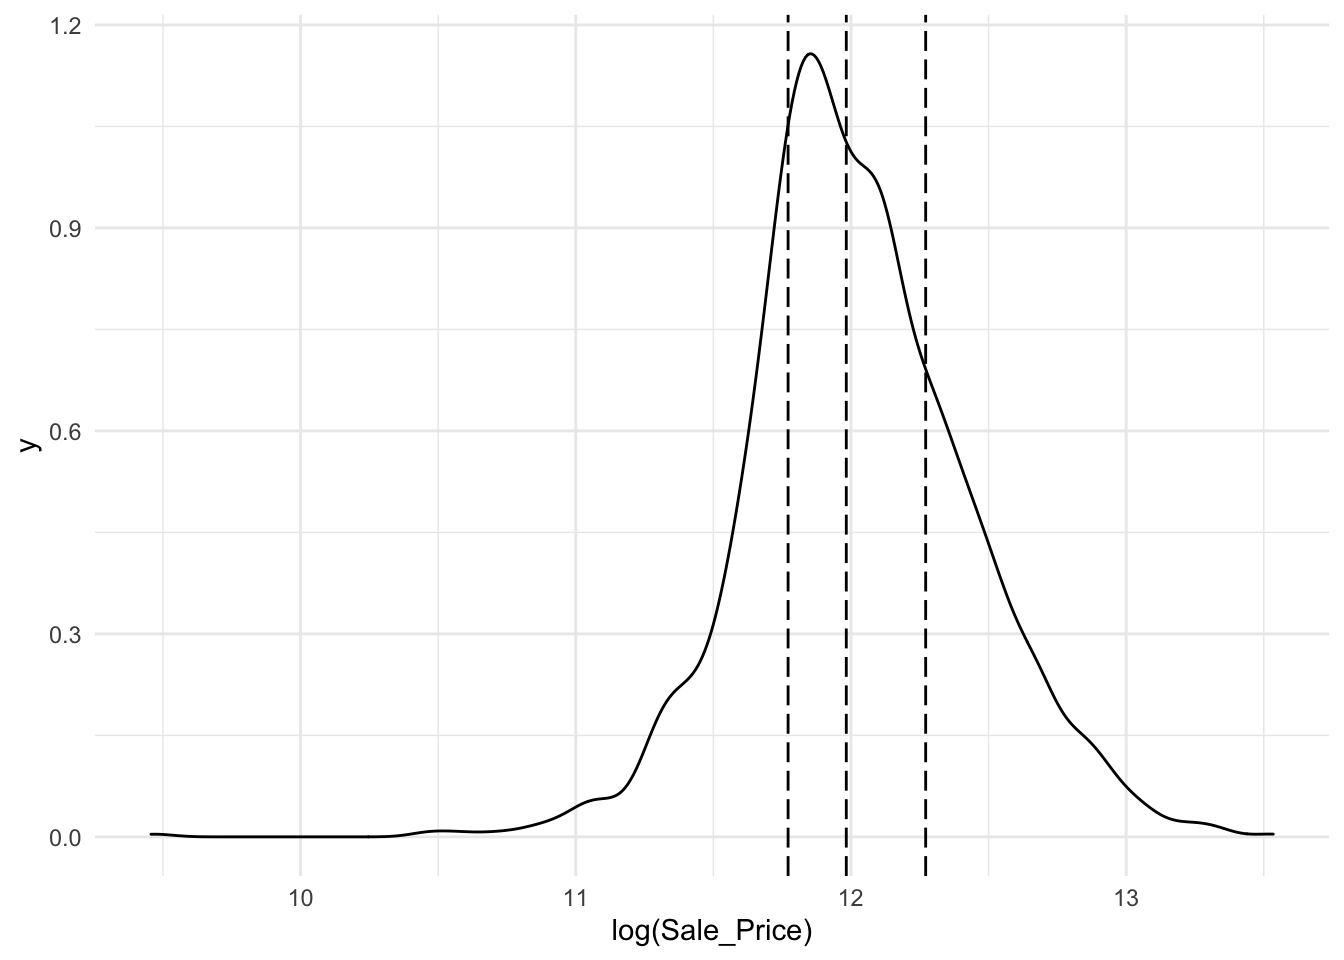
\includegraphics{amt22_03intro2mls2_files/figure-latex/unnamed-chunk-38-1.pdf}

Observamos que la distribución del precio de venta está sesgada a la derecha.
Las casas más caras no estarían bien representadas en el conjunto de entrenamiento con una simple partición; esto aumentaría el riesgo de que nuestro modelo sea ineficaz para predecir el precio de dichas propiedades.

Las líneas verticales punteadas indican los cuatro cuartiles para estos datos.
Una muestra aleatoria estratificada llevaría a cabo la división 80/20 dentro de cada uno de estos subconjuntos de datos y luego combinaría los resultados. En \emph{rsample}, esto se logra usando el argumento de estratos:

\begin{Shaded}
\begin{Highlighting}[]
\FunctionTok{set.seed}\NormalTok{(}\DecValTok{123}\NormalTok{)}
\NormalTok{ames\_split }\OtherTok{\textless{}{-}} \FunctionTok{initial\_split}\NormalTok{(ames, }\AttributeTok{prop =} \FloatTok{0.80}\NormalTok{, }\AttributeTok{strata =}\NormalTok{ Sale\_Price)}
\NormalTok{ames\_train }\OtherTok{\textless{}{-}} \FunctionTok{training}\NormalTok{(ames\_split)}
\NormalTok{ames\_test  }\OtherTok{\textless{}{-}}  \FunctionTok{testing}\NormalTok{(ames\_split)}
\end{Highlighting}
\end{Shaded}

\textbf{Hay muy pocas desventajas en el uso de muestreo estratificado.}

Un caso es cuando los datos tienen un componente de tiempo, como los datos de series de tiempo.
Aquí, es más común utilizar los datos más recientes como conjunto de prueba.

El paquete \emph{rsample} contiene una función llamada \texttt{initial\_time\_split()}
que es muy similar a \texttt{initial\_split()}. En lugar de usar un muestreo aleatorio, el argumento \texttt{prop}
denota qué proporción de la primera parte de los datos debe usarse como conjunto de entrenamiento;
la función asume que los datos se han clasificado previamente en un orden apropiado.

\hypertarget{quuxe9-proporciuxf3n-deberuxeda-ser-usada}{%
\subsection{¿Qué proporción debería ser usada?}\label{quuxe9-proporciuxf3n-deberuxeda-ser-usada}}

No hay un porcentaje de división óptimo para el conjunto de entrenamiento y prueba.
Muy pocos datos en el conjunto de entrenamiento obstaculizan la capacidad del modelo para encontrar estimaciones de parámetros adecuadas y muy pocos datos en el conjunto de prueba reducen la calidad de las estimaciones de rendimiento.

Se debe elegir un porcentaje que cumpla con los objetivos de nuestro proyecto con consideraciones que incluyen:

\begin{itemize}
\tightlist
\item
  Costo computacional en el entrenamiento del modelo.
\item
  Costo computacional en la evaluación del modelo.
\item
  Representatividad del conjunto de formación.
\item
  Representatividad del conjunto de pruebas.
\end{itemize}

Los porcentajes de división más comunes comunes son:

\begin{itemize}
\tightlist
\item
  Entrenamiento: \(80\%\), Prueba: \(20\%\)
\item
  Entrenamiento: \(67\%\), Prueba: \(33\%\)
\item
  Entrenamiento: \(50\%\), Prueba: \(50\%\)
\end{itemize}

\hypertarget{conjunto-de-validaciuxf3n}{%
\subsection{Conjunto de validación}\label{conjunto-de-validaciuxf3n}}

El conjunto de validación se definió originalmente cuando los investigadores se dieron cuenta de que medir el rendimiento del conjunto de entrenamiento conducía a resultados que eran demasiado optimistas.

Esto llevó a modelos que se sobreajustaban, lo que significa que se desempeñaron muy bien en el conjunto de entrenamiento pero mal en el conjunto de prueba.

Para combatir este problema, se retuvo un pequeño conjunto de datos de \emph{validación} y se utilizó para medir el rendimiento del modelo mientras este está siendo entrenado. Una vez que la tasa de error del conjunto de validación comenzara a aumentar, la capacitación se detendría.

En otras palabras, el conjunto de validación es un medio para tener una idea aproximada de qué tan bien se desempeñó el modelo antes del conjunto de prueba.

\begin{center}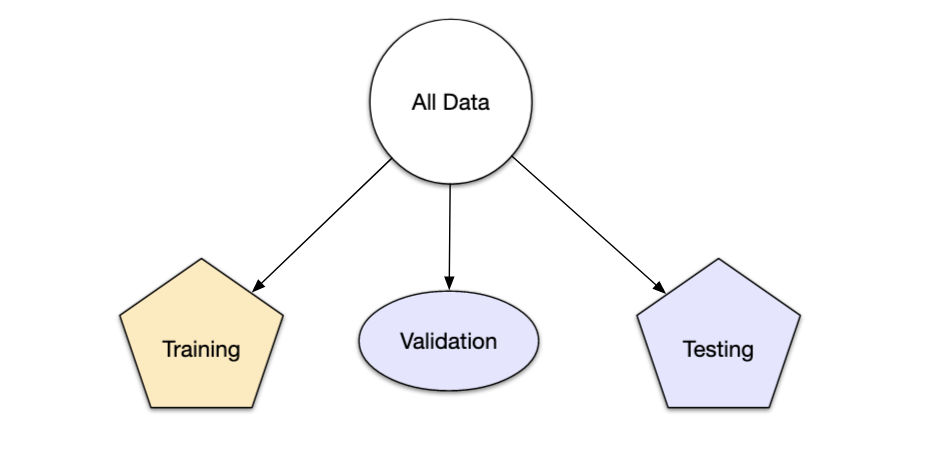
\includegraphics[width=500pt,height=250pt]{img/04-ml/3-5-3-conjunto-validacion} \end{center}

Los conjuntos de validación se utilizan a menudo cuando el conjunto de datos original es muy grande. En este caso, una sola partición grande puede ser adecuada para caracterizar el rendimiento del modelo sin tener que realizar múltiples iteraciones de remuestreo.

Con \emph{rsample}, un conjunto de validación es como cualquier otro objeto de remuestreo; este tipo es diferente solo en que tiene una sola iteración

\begin{center}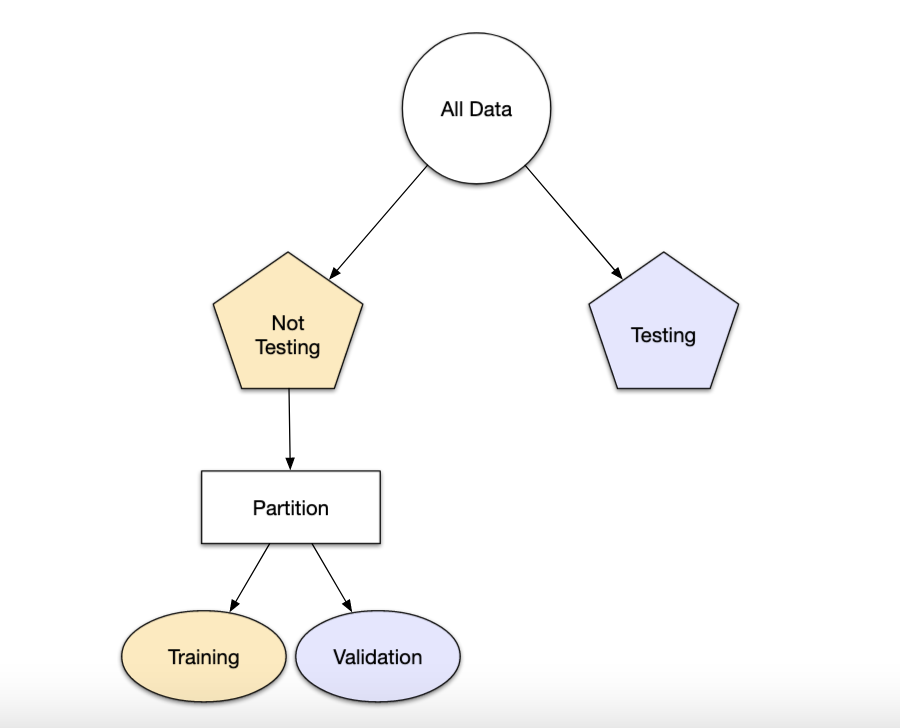
\includegraphics[width=500pt,height=350pt]{img/04-ml/3-5-3-conjunto-validacion-2} \end{center}

\begin{Shaded}
\begin{Highlighting}[]
\FunctionTok{set.seed}\NormalTok{(}\DecValTok{12}\NormalTok{)}
\NormalTok{val\_set }\OtherTok{\textless{}{-}} \FunctionTok{validation\_split}\NormalTok{(ames\_train, }\AttributeTok{prop =} \DecValTok{3}\SpecialCharTok{/}\DecValTok{4}\NormalTok{, }\AttributeTok{strata =} \ConstantTok{NULL}\NormalTok{)}
\NormalTok{val\_set }\CommentTok{\#val\_set contiene el conjunto de entrenamiento y validación.}
\end{Highlighting}
\end{Shaded}

\begin{verbatim}
## # Validation Set Split (0.75/0.25)  
## # A tibble: 1 x 2
##   splits             id        
##   <list>             <chr>     
## 1 <split [1756/586]> validation
\end{verbatim}

Esta función regresa una columna para los objetos de división de datos y una columna llamada id que tiene una cadena de caracteres con el identificador de remuestreo.

El argumento de estratos hace que el muestreo aleatorio se lleve a cabo dentro de la variable de estratificación. Esto puede ayudar a garantizar que el número de datos en los datos del análisis sea equivalente a las proporciones del conjunto de datos original. (Los estratos inferiores al 10\% del total se agrupan).

Otra opción de muestreo bastante común es la realizada mediante múltiples submuestras de los datos originales.

\begin{center}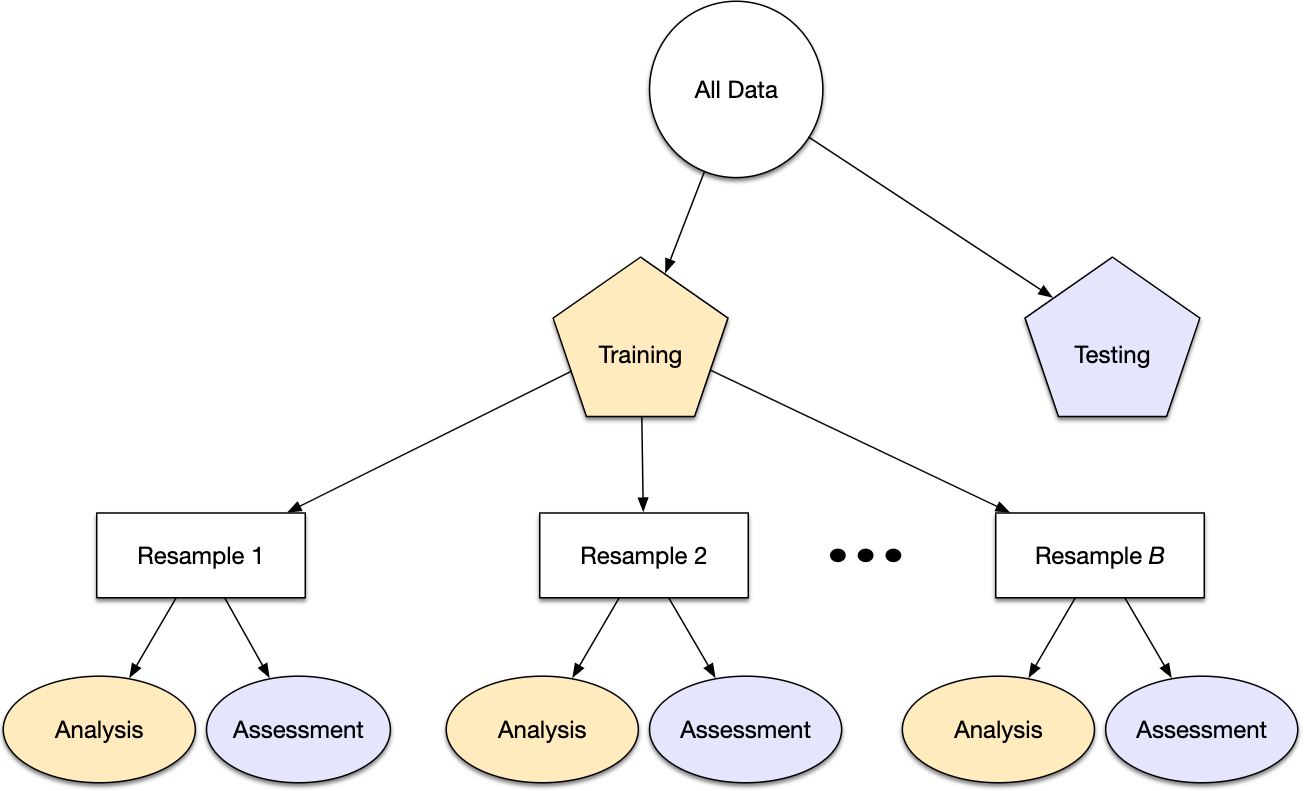
\includegraphics[width=500pt,height=350pt]{img/04-ml/18_1_cross_validation} \end{center}

Diversos métodos se revisarán a lo largo del curso.

\hypertarget{leave-one-out-cross-validation}{%
\subsection{Leave-one-out cross-validation}\label{leave-one-out-cross-validation}}

La validación cruzada es una manera de predecir el ajuste de un modelo a un hipotético conjunto de datos de prueba cuando no disponemos del conjunto explícito de datos de prueba.

El método \emph{LOOCV} en un método iterativo que se inicia empleando como conjunto
de entrenamiento todas las observaciones disponibles excepto una, que se excluye
para emplearla como validación.

Si se emplea una única observación para calcular el error, este varía mucho
dependiendo de qué observación se haya seleccionado. Para evitarlo, el proceso
se repite tantas veces como observaciones disponibles se tengan, excluyendo en
cada iteración una observación distinta, ajustando el modelo con el resto y
calculando el error con dicha observación.

Finalmente, el error estimado por el es el promedio de todos lo \(i\) errores calculados.

La principal desventaja de este método es su costo computacional.
El proceso requiere que el modelo sea reajustado y validado tantas veces como observaciones disponibles
se tengan lo que en algunos casos puede ser muy complicado.

\emph{rsample} contiene la función \texttt{loo\_cv()}.

\begin{Shaded}
\begin{Highlighting}[]
\FunctionTok{set.seed}\NormalTok{(}\DecValTok{55}\NormalTok{)}
\NormalTok{ames\_loo }\OtherTok{\textless{}{-}} \FunctionTok{loo\_cv}\NormalTok{(ames\_train)}
\NormalTok{ames\_loo}
\end{Highlighting}
\end{Shaded}

\begin{verbatim}
## # Leave-one-out cross-validation 
## # A tibble: 2,342 x 2
##    splits           id        
##    <list>           <chr>     
##  1 <split [2341/1]> Resample1 
##  2 <split [2341/1]> Resample2 
##  3 <split [2341/1]> Resample3 
##  4 <split [2341/1]> Resample4 
##  5 <split [2341/1]> Resample5 
##  6 <split [2341/1]> Resample6 
##  7 <split [2341/1]> Resample7 
##  8 <split [2341/1]> Resample8 
##  9 <split [2341/1]> Resample9 
## 10 <split [2341/1]> Resample10
## # ... with 2,332 more rows
\end{verbatim}

\hypertarget{support-vector-machine-svm}{%
\chapter{Support Vector Machine (SVM)}\label{support-vector-machine-svm}}

Support vector machine, llamadas SVM, son un algoritmo de aprendizaje supervisado que se puede utilizar para problemas de clasificación y regresión. Se utiliza para conjuntos de datos más pequeños, ya que tarda demasiado en procesarse.

\begin{center}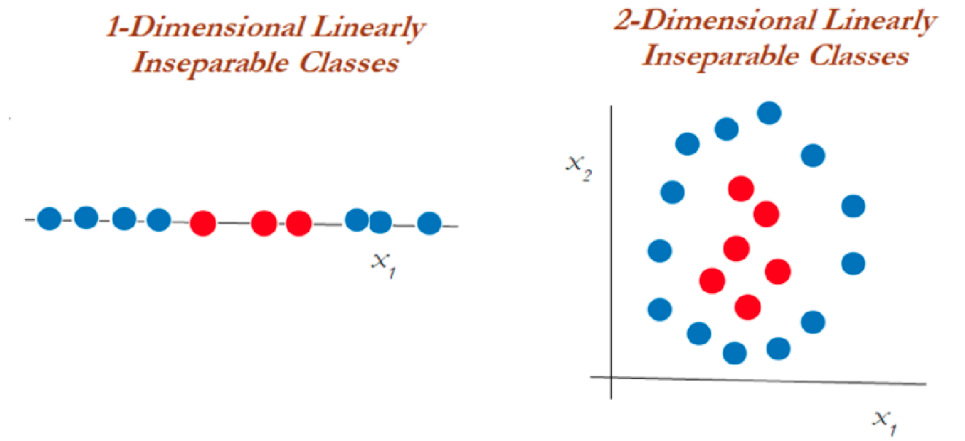
\includegraphics[width=800pt,height=400pt]{img/02-svm/01_inseparable_classes} \end{center}

El principal objetivo de esta técnica es encontrar el \textbf{Hiperplano de Separación Óptima}, también conocido como \emph{Boundary Decision}, el cual separa a las clases involucradas.

Para entender este algoritmo es necesario entender 3 conceptos principales:

\begin{quote}
\begin{enumerate}
\def\labelenumi{\arabic{enumi}.}
\tightlist
\item
  Maximum margin classifiers
\end{enumerate}
\end{quote}

\begin{quote}
\begin{enumerate}
\def\labelenumi{\arabic{enumi}.}
\setcounter{enumi}{1}
\tightlist
\item
  Support vector classifiers
\end{enumerate}
\end{quote}

\begin{quote}
\begin{enumerate}
\def\labelenumi{\arabic{enumi}.}
\setcounter{enumi}{2}
\tightlist
\item
  Support vector machines
\end{enumerate}
\end{quote}

Estudiemos cada uno de estos principios.

\hypertarget{maximum-margin-classifier}{%
\section{Maximum Margin Classifier}\label{maximum-margin-classifier}}

A menudo se generalizan con máquinas de vectores de soporte, pero SVM tiene muchos más parámetros en comparación. El \emph{clasificador de margen máximo} considera un hiperplano con ancho de separación máxima para clasificar los datos. Sin embargo, se pueden dibujar infinitos hiperplanos en un conjunto de datos por lo que es importante elegir el hiperplano ideal para la clasificación.

En un espacio \emph{n-dimensional}, un hiperplano es un subespacio de la dimensión n-1. Es decir, si los datos tienen un espacio bidimensional, entonces el hiperplano puede ser una línea recta que divide el espacio de datos en dos mitades y pasa por la siguiente ecuacion:

\[\beta_0 + \beta_1X_1 + \beta_2X_2=0\]

Las observaciones que caen en el hiperplano sigue la ecuación anterior. Las observaciones que caen en la región por encima o por debajo del hiperplano sigue las siguientes ecuaciones:

\[\beta_0 + \beta_1X_1 + \beta_2X_2>0\]

\[\beta_0 + \beta_1X_1 + \beta_2X_2<0\]

El clasificador de margen máximo a menudo falla en la situación de casos no separables en los que no puede asignar un hiperplano diferente para clasificar datos no separables. Para tales casos, un clasificador de vectores de soporte viene al rescate.

\begin{center}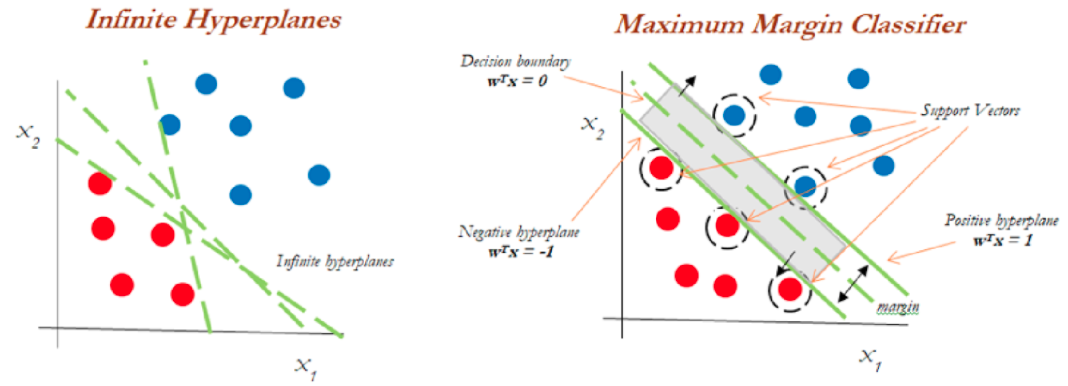
\includegraphics[width=900pt,height=380pt]{img/02-svm/02_maximum_margin_classifier} \end{center}

Del diagrama anterior, podemos suponer infinitos hiperplanos (izquierda). El clasificador de margen máximo viene con un solo hiperplano que divide los datos como en la gráfica de la derecha. \textbf{Los datos que tocan los hiperplanos positivo y negativo se denominan vectores de soporte}.

\hypertarget{support-vector-classifiers}{%
\section{Support Vector Classifiers}\label{support-vector-classifiers}}

\textbf{Los vectores de soporte son las observaciones que están más cerca del hiperplano e influyen en la posición y orientación del hiperplano}. Este tipo de clasificador puede considerarse como una versión extendida del clasificador de margen máximo. Cuando tratamos con datos de la vida real, encontramos que la mayoría de las observaciones están en clases superpuestas. Es por eso que se implementan clasificadores de vectores de soporte.

Usando estos vectores de soporte, maximizamos el margen del clasificador. Eliminar los vectores de soporte cambiará la posición del hiperplano. Estos son los puntos que nos ayudan a construir nuestro \emph{SVM}. Consideremos un \textbf{parámetro de ajuste C}. En este clasificador, el alto valor de \emph{C} puede darnos un modelo robusto. Un valor más bajo de \emph{C} nos da un modelo flexible. Entendamos con el siguiente diagrama.

\begin{center}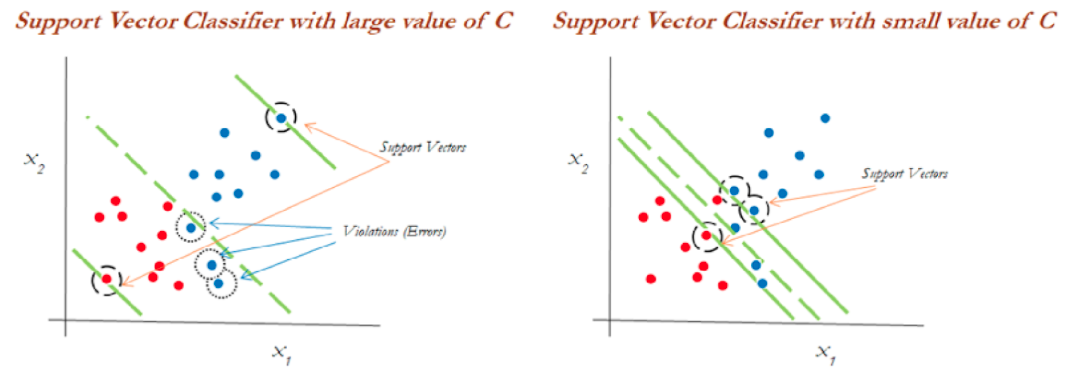
\includegraphics[width=900pt,height=380pt]{img/02-svm/03_support_vector_classifier} \end{center}

Podemos ver en el gráfico de la izquierda que los valores más altos de \emph{C} generaron más errores que se consideran una \textbf{violación o infracción}. El diagrama de la derecha muestra un valor más bajo de \emph{C} y no brinda suficientes posibilidades de infracción al reducir el ancho del margen.

\hypertarget{support-vector-machine}{%
\section{Support Vector Machine}\label{support-vector-machine}}

El enfoque de la máquina de vectores de soporte se considera durante una decisión no lineal y los datos no son separables por un clasificador de vectores de soporte, independientemente de la función de costo.

Cuando es casi imposible separar clases de manera no lineal, aplicamos el truco llamado \textbf{truco del kernel} el cual ayuda a manejar la separación de los datos.

\begin{center}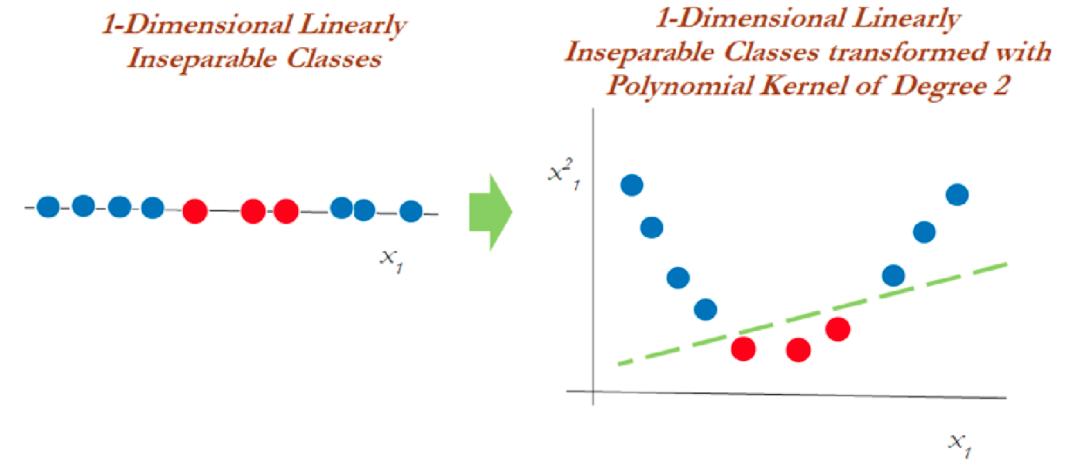
\includegraphics[width=900pt,height=380pt]{img/02-svm/04_polinomial_kernel_plot} \end{center}

En el gráfico anterior, los datos que eran inseparables en una dimensión se separaron una vez que se transformaron a un espacio de dos dimensiones después de aplicar una \textbf{transformación mediante kernel polinomial de segundo grado}. Ahora veamos cómo manejar los datos bidimensionales linealmente inseparables.

\begin{center}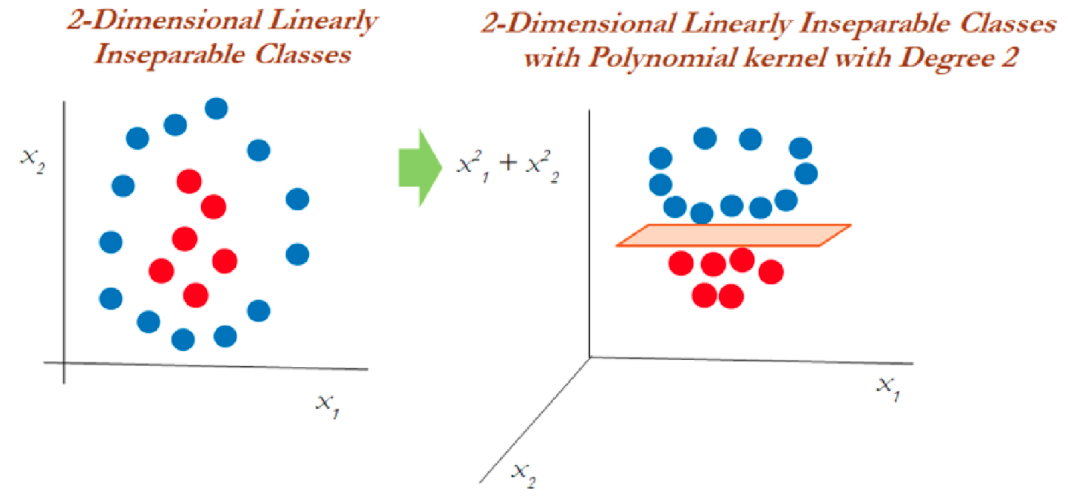
\includegraphics[width=900pt,height=380pt]{img/02-svm/05_kernel_polinomial_plot2} \end{center}

En datos bidimensionales, el núcleo polinomial de segundo grado se aplica utilizando un plano lineal después de transformarlo a dimensiones superiores.

\hypertarget{el-truco-del-kernel}{%
\section{El truco del Kernel}\label{el-truco-del-kernel}}

Las funciones Kernel son métodos con los que se utilizan clasificadores lineales como \emph{SVM} para clasificar puntos de datos separables no linealmente. Esto se hace representando los puntos de datos en un espacio de mayor dimensión que su original. Por ejemplo, los datos 1D se pueden representar como datos 2D en el espacio, los datos 2D se pueden representar como datos 3D, etcétera.

El truco del kernel ofrece una \textbf{forma de calcular las relaciones entre los puntos de datos} utilizando funciones del kernel y representar los datos de una manera más eficiente con menos cómputo. Los modelos que utilizan esta técnica se denominan \textbf{``modelos kernelizados''}.

\begin{center}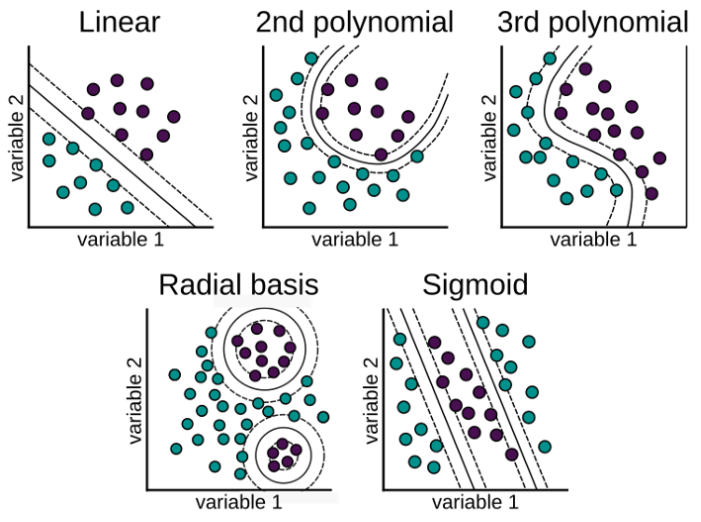
\includegraphics[width=700pt,height=500pt]{img/02-svm/06_kernels} \end{center}

Hay varias funciones que utiliza SVM para realizar esta tarea. Algunos de los más comunes son:

\begin{enumerate}
\def\labelenumi{\arabic{enumi}.}
\tightlist
\item
  \textbf{El núcleo lineal:} Se utiliza para datos lineales. Esto simplemente representa los puntos de datos usando una relación lineal.
\end{enumerate}

\[K(x, y)=(x^T \cdot y)\]
\[f(x)=w^T \cdot x + b\]
Esta formulación se presenta como solución al problema de optimización sobre w:

\[min_{w\in R^d} \parallel w \parallel ^2+ C\sum_{i}^{N}{max(0, 1-y_if(x_i))}\]
\[s.a. \quad y_i(w^T x_i+b) \geq 1 - max(0, 1-y_if(x_i))\]

\begin{enumerate}
\def\labelenumi{\arabic{enumi}.}
\setcounter{enumi}{1}
\tightlist
\item
  \textbf{Función de núcleo polinomial:} Transforma los puntos de datos mediante el \textbf{uso del producto escalar} y la transformación de los datos en una ``dimensión \emph{n}'', \emph{n} podría ser cualquier valor de 2, 3, etcétera, es decir, la transformación será un producto al cuadrado o superior. Por lo tanto, representar datos en un espacio de mayor dimensión utilizando los nuevos puntos transformados.
\end{enumerate}

\[K(x, y)=(c+ x^T \cdot y)^p\]

Cuando se emplea \(p=1\) y \(c=0\), el resultado es el mismo que el de un kernel lineal. Si \(p>1\), se generan límites de decisión no lineales, aumentando la no linealidad a medida que aumenta \emph{p}. No suele ser recomendable emplear valores de \emph{p} mayores 5 por problemas de \textbf{overfitting}.

\begin{center}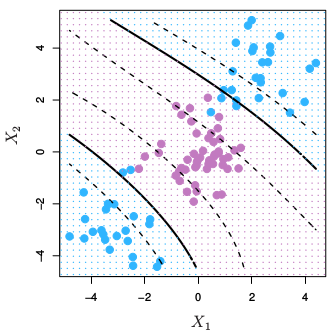
\includegraphics[width=400pt,height=400pt]{img/02-svm/3-15-1-poli} \end{center}

\begin{enumerate}
\def\labelenumi{\arabic{enumi}.}
\setcounter{enumi}{2}
\tightlist
\item
  \textbf{La función de base radial (RBF):} Esta función se comporta como un ``modelo de vecino más cercano ponderado''. Transforma los datos representándolos en dimensiones infinitas,
\end{enumerate}

La función Radial puede ser de Gauss o de Laplace. Esto depende de un hiperparámetro conocido como gamma \(\gamma\). Cuanto menor sea el valor del hiperparámetro, menor será el sesgo y mayor la varianza. Mientras que un valor más alto de hiperparámetro da un sesgo más alto y menor varianza. Este es el núcleo más utilizado.

\[K(x, y)=exp(-\gamma \parallel x - y\parallel^2)=exp(-\frac{\parallel x-y \parallel ^2}{2\sigma²})\]
\[f(x)=w^T \cdot \phi(x) + b\]
Se realiza un mapeo de x a \(\phi(x)\) en donde los datos son separables

\begin{center}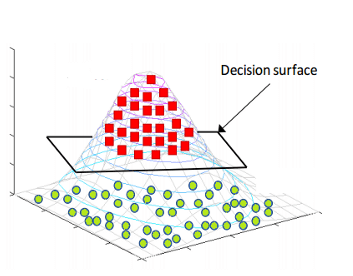
\includegraphics[width=400pt,height=400pt]{img/02-svm/svm_radial} \end{center}

Es recomendable probar el kernel \textbf{RBF}. Este kernel tiene dos ventajas: que solo tiene dos hiperparámetros que optimizar (\(\gamma\) y la penalización \(C\) común a todos los SVM) y que su flexibilidad puede ir desde un clasificador lineal a uno muy complejo.

\begin{enumerate}
\def\labelenumi{\arabic{enumi}.}
\setcounter{enumi}{3}
\tightlist
\item
  \textbf{La función sigmoide:} También conocida como función tangente hiperbólica (Tanh), encuentra más aplicación en redes neuronales como función de activación. Esta función se utiliza en la clasificación de imágenes.
\end{enumerate}

\[K(x, y)= tanh(\kappa x\cdot y-\delta)\]

¿Por qué se llama un ``truco del kernel''? \emph{SVM} vuelve a representar hábilmente los puntos de datos no lineales utilizando cualquiera de las funciones del kernel de una manera que parece que los datos se han transformado, luego encuentra el hiperplano de separación óptimo. Sin embargo, en realidad, los puntos de datos siguen siendo los mismos, en realidad no se han transformado. Es por eso que se llama un `truco del kernel'.

\hypertarget{ventajas-y-desventajas}{%
\section{Ventajas y desventajas}\label{ventajas-y-desventajas}}

\textbf{Ventajas}

\begin{itemize}
\item
  Es un modelo que ajusta bien con pocos datos
\item
  Son flexibles en datos no estructurados, estructurados y semiestructurados.
\item
  La función Kernel alivia las complejidades en casi cualquier tipo de datos.
\item
  Se observa menos sobreajuste en comparación con otros modelos.
\end{itemize}

\textbf{Desventajas}

\begin{itemize}
\item
  El tiempo de entrenamiento es mayor cuando se calculan grandes conjuntos de datos.
\item
  Los hiperparámetros suelen ser un desafío al interpretar su impacto.
\item
  La interpretación general es difícil (black box).
\end{itemize}

\hypertarget{ajuste-del-modelo-con-r}{%
\section{Ajuste del modelo con R}\label{ajuste-del-modelo-con-r}}

Usaremos las recetas antes implementadas para ajustar tanto el modelo de regresión como el de clasificación. Exploraremos un conjunto de hiperparámetros para elegir el mejor modelo.

Recordemos que es importante separar los datos de entrenamiento y prueba, así como sub-particionar en fold a los datos de entrenamiento para realizar diferentes pruebas con distintas parametrizaciones de los modelos. Finalmente, calcularemos el error promedio y los mejores hiperparámetros a implementar.

\begin{Shaded}
\begin{Highlighting}[]
\FunctionTok{library}\NormalTok{(tidymodels)}

\FunctionTok{data}\NormalTok{(ames)}

\FunctionTok{set.seed}\NormalTok{(}\DecValTok{4595}\NormalTok{)}
\NormalTok{ames\_split }\OtherTok{\textless{}{-}} \FunctionTok{initial\_split}\NormalTok{(ames, }\AttributeTok{prop =} \FloatTok{0.75}\NormalTok{)}
\NormalTok{ames\_train }\OtherTok{\textless{}{-}} \FunctionTok{training}\NormalTok{(ames\_split)}
\NormalTok{ames\_test  }\OtherTok{\textless{}{-}} \FunctionTok{testing}\NormalTok{(ames\_split)}
\NormalTok{ames\_folds}\OtherTok{\textless{}{-}} \FunctionTok{vfold\_cv}\NormalTok{(ames\_train)}
\end{Highlighting}
\end{Shaded}

Contando con datos de entrenamiento, procedemos a realizar el feature engineering para extraer las mejores características que permitirán realizar las estimaciones en el modelo.

\begin{Shaded}
\begin{Highlighting}[]
\NormalTok{receta\_casas }\OtherTok{\textless{}{-}} \FunctionTok{recipe}\NormalTok{(Sale\_Price }\SpecialCharTok{\textasciitilde{}}\NormalTok{ . , }\AttributeTok{data =}\NormalTok{ ames\_train) }\SpecialCharTok{\%\textgreater{}\%}
  \FunctionTok{step\_unknown}\NormalTok{(Alley) }\SpecialCharTok{\%\textgreater{}\%}
  \FunctionTok{step\_rename}\NormalTok{(}\AttributeTok{Year\_Remod =}\NormalTok{ Year\_Remod\_Add) }\SpecialCharTok{\%\textgreater{}\%} 
  \FunctionTok{step\_rename}\NormalTok{(}\AttributeTok{ThirdSsn\_Porch =}\NormalTok{ Three\_season\_porch) }\SpecialCharTok{\%\textgreater{}\%} 
  \FunctionTok{step\_ratio}\NormalTok{(Bedroom\_AbvGr, }\AttributeTok{denom =} \FunctionTok{denom\_vars}\NormalTok{(Gr\_Liv\_Area)) }\SpecialCharTok{\%\textgreater{}\%} 
  \FunctionTok{step\_mutate}\NormalTok{(}
    \AttributeTok{Age\_House =}\NormalTok{ Year\_Sold }\SpecialCharTok{{-}}\NormalTok{ Year\_Remod,}
    \AttributeTok{TotalSF   =}\NormalTok{ Gr\_Liv\_Area }\SpecialCharTok{+}\NormalTok{ Total\_Bsmt\_SF,}
    \AttributeTok{AvgRoomSF   =}\NormalTok{ Gr\_Liv\_Area }\SpecialCharTok{/}\NormalTok{ TotRms\_AbvGrd,}
    \AttributeTok{Pool =} \FunctionTok{if\_else}\NormalTok{(Pool\_Area }\SpecialCharTok{\textgreater{}} \DecValTok{0}\NormalTok{, }\DecValTok{1}\NormalTok{, }\DecValTok{0}\NormalTok{),}
    \AttributeTok{Exter\_Cond =}\NormalTok{ forcats}\SpecialCharTok{::}\FunctionTok{fct\_collapse}\NormalTok{(Exter\_Cond, }\AttributeTok{Good =} \FunctionTok{c}\NormalTok{(}\StringTok{"Typical"}\NormalTok{, }\StringTok{"Good"}\NormalTok{, }\StringTok{"Excellent"}\NormalTok{))) }\SpecialCharTok{\%\textgreater{}\%} 
  \FunctionTok{step\_relevel}\NormalTok{(Exter\_Cond, }\AttributeTok{ref\_level =} \StringTok{"Good"}\NormalTok{) }\SpecialCharTok{\%\textgreater{}\%} 
  \FunctionTok{step\_normalize}\NormalTok{(}\FunctionTok{all\_predictors}\NormalTok{(), }\SpecialCharTok{{-}}\FunctionTok{all\_nominal}\NormalTok{()) }\SpecialCharTok{\%\textgreater{}\%}
  \FunctionTok{step\_dummy}\NormalTok{(}\FunctionTok{all\_nominal}\NormalTok{()) }\SpecialCharTok{\%\textgreater{}\%} 
  \FunctionTok{step\_interact}\NormalTok{(}\SpecialCharTok{\textasciitilde{}}\NormalTok{ Second\_Flr\_SF}\SpecialCharTok{:}\NormalTok{First\_Flr\_SF) }\SpecialCharTok{\%\textgreater{}\%} 
  \FunctionTok{step\_interact}\NormalTok{(}\SpecialCharTok{\textasciitilde{}} \FunctionTok{matches}\NormalTok{(}\StringTok{"Bsmt\_Cond"}\NormalTok{)}\SpecialCharTok{:}\NormalTok{TotRms\_AbvGrd) }\SpecialCharTok{\%\textgreater{}\%} 
  \FunctionTok{step\_rm}\NormalTok{(}
\NormalTok{    First\_Flr\_SF, Second\_Flr\_SF, Year\_Remod,}
\NormalTok{    Bsmt\_Full\_Bath, Bsmt\_Half\_Bath, }
\NormalTok{    Kitchen\_AbvGr, BsmtFin\_Type\_1\_Unf, }
\NormalTok{    Total\_Bsmt\_SF, Kitchen\_AbvGr, Pool\_Area, }
\NormalTok{    Gr\_Liv\_Area, Sale\_Type\_Oth, Sale\_Type\_VWD}
\NormalTok{  ) }\SpecialCharTok{\%\textgreater{}\%} 
  \FunctionTok{prep}\NormalTok{()}
\end{Highlighting}
\end{Shaded}

Recordemos que la función \textbf{recipe()} solo son los pasos a seguir, necesitamos usar la función \textbf{prep()} que nos devuelve una receta actualizada con las estimaciones y la función \textbf{juice()} que nos devuelve la matriz de diseño.

Una vez que la receta de transformación de datos está lista, procedemos a implementar el pipeline del modelo de interés.

\begin{Shaded}
\begin{Highlighting}[]
\NormalTok{svm\_model }\OtherTok{\textless{}{-}} \FunctionTok{svm\_rbf}\NormalTok{(}
  \AttributeTok{mode =} \StringTok{"regression"}\NormalTok{,}
  \AttributeTok{cost =} \FunctionTok{tune}\NormalTok{(),}
  \AttributeTok{rbf\_sigma =} \FunctionTok{tune}\NormalTok{(),}
  \AttributeTok{margin =} \FunctionTok{tune}\NormalTok{()) }\SpecialCharTok{\%\textgreater{}\%} 
\FunctionTok{set\_engine}\NormalTok{(}\StringTok{"kernlab"}\NormalTok{)}

\NormalTok{svm\_workflow }\OtherTok{\textless{}{-}} \FunctionTok{workflow}\NormalTok{() }\SpecialCharTok{\%\textgreater{}\%} 
  \FunctionTok{add\_recipe}\NormalTok{(receta\_casas) }\SpecialCharTok{\%\textgreater{}\%} 
  \FunctionTok{add\_model}\NormalTok{(svm\_model)}

\NormalTok{svm\_parameters\_set }\OtherTok{\textless{}{-}} \FunctionTok{parameters}\NormalTok{(svm\_workflow) }\SpecialCharTok{\%\textgreater{}\%} 
  \FunctionTok{update}\NormalTok{(}
   \AttributeTok{rbf\_sigma =} \FunctionTok{rbf\_sigma}\NormalTok{(}\FunctionTok{c}\NormalTok{(}\SpecialCharTok{{-}}\FloatTok{2.5}\NormalTok{, }\FloatTok{2.5}\NormalTok{)), }
   \AttributeTok{cost =} \FunctionTok{cost}\NormalTok{(}\FunctionTok{c}\NormalTok{(}\DecValTok{0}\NormalTok{, }\DecValTok{15}\NormalTok{))}
\NormalTok{   )}

\FunctionTok{set.seed}\NormalTok{(}\DecValTok{123}\NormalTok{)}
\NormalTok{svm\_grid }\OtherTok{\textless{}{-}}\NormalTok{ svm\_parameters\_set }\SpecialCharTok{\%\textgreater{}\%} 
  \FunctionTok{grid\_max\_entropy}\NormalTok{(}\AttributeTok{size =} \DecValTok{80}\NormalTok{)}

\NormalTok{ctrl\_grid }\OtherTok{\textless{}{-}} \FunctionTok{control\_grid}\NormalTok{(}\AttributeTok{save\_pred =}\NormalTok{ T, }\AttributeTok{verbose =}\NormalTok{ T)}
\end{Highlighting}
\end{Shaded}

\begin{Shaded}
\begin{Highlighting}[]
\FunctionTok{library}\NormalTok{(doParallel)}

\NormalTok{UseCores }\OtherTok{\textless{}{-}} \FunctionTok{detectCores}\NormalTok{() }\SpecialCharTok{{-}} \DecValTok{1}
\NormalTok{cluster }\OtherTok{\textless{}{-}} \FunctionTok{makeCluster}\NormalTok{(UseCores)}
\FunctionTok{registerDoParallel}\NormalTok{(cluster)}

\NormalTok{svm1 }\OtherTok{\textless{}{-}} \FunctionTok{Sys.time}\NormalTok{()}
\NormalTok{svm\_tune\_result }\OtherTok{\textless{}{-}} \FunctionTok{tune\_grid}\NormalTok{(}
\NormalTok{  svm\_workflow,}
  \AttributeTok{resamples =}\NormalTok{ ames\_folds,}
  \AttributeTok{grid =}\NormalTok{ svm\_grid,}
  \AttributeTok{metrics =} \FunctionTok{metric\_set}\NormalTok{(rmse, mae, mape),}
  \AttributeTok{control =}\NormalTok{ ctrl\_grid}
\NormalTok{)}
\NormalTok{svm2 }\OtherTok{\textless{}{-}} \FunctionTok{Sys.time}\NormalTok{(); svm2 }\SpecialCharTok{{-}}\NormalTok{ svm1}

\FunctionTok{stopCluster}\NormalTok{(cluster)}

\NormalTok{svm\_tune\_result }\SpecialCharTok{\%\textgreater{}\%} \FunctionTok{saveRDS}\NormalTok{(}\StringTok{"models/svm\_model\_reg.rds"}\NormalTok{)}
\end{Highlighting}
\end{Shaded}

Podemos obtener las métricas de cada \emph{fold} con el siguiente código:

\begin{Shaded}
\begin{Highlighting}[]
\NormalTok{svm\_tune\_result }\OtherTok{\textless{}{-}} \FunctionTok{readRDS}\NormalTok{(}\StringTok{"models/svm\_model\_reg.rds"}\NormalTok{)}

\NormalTok{svm\_tune\_result }\SpecialCharTok{\%\textgreater{}\%} \FunctionTok{unnest}\NormalTok{(.metrics)}
\end{Highlighting}
\end{Shaded}

\begin{verbatim}
## # A tibble: 2,400 x 11
##    splits             id      cost rbf_sigma margin .metric .estimator .estimate
##    <list>             <chr>  <dbl>     <dbl>  <dbl> <chr>   <chr>          <dbl>
##  1 <split [1977/220]> Fold~   357.    0.0839 0.110  rmse    standard     43741. 
##  2 <split [1977/220]> Fold~   357.    0.0839 0.110  mae     standard     28240. 
##  3 <split [1977/220]> Fold~   357.    0.0839 0.110  mape    standard        18.6
##  4 <split [1977/220]> Fold~ 10956.    5.22   0.180  rmse    standard     90721. 
##  5 <split [1977/220]> Fold~ 10956.    5.22   0.180  mae     standard     66139. 
##  6 <split [1977/220]> Fold~ 10956.    5.22   0.180  mape    standard        42.4
##  7 <split [1977/220]> Fold~  5733.   96.0    0.0128 rmse    standard     91135. 
##  8 <split [1977/220]> Fold~  5733.   96.0    0.0128 mae     standard     65465. 
##  9 <split [1977/220]> Fold~  5733.   96.0    0.0128 mape    standard        41.4
## 10 <split [1977/220]> Fold~ 26216.    7.45   0.197  rmse    standard     90721. 
## # ... with 2,390 more rows, and 3 more variables: .config <chr>, .notes <list>,
## #   .predictions <list>
\end{verbatim}

En la siguiente gráfica observamos el error cuadrático medio de las distintas métricas:

\begin{Shaded}
\begin{Highlighting}[]
\NormalTok{svm\_tune\_result }\SpecialCharTok{\%\textgreater{}\%} \FunctionTok{autoplot}\NormalTok{()}
\end{Highlighting}
\end{Shaded}

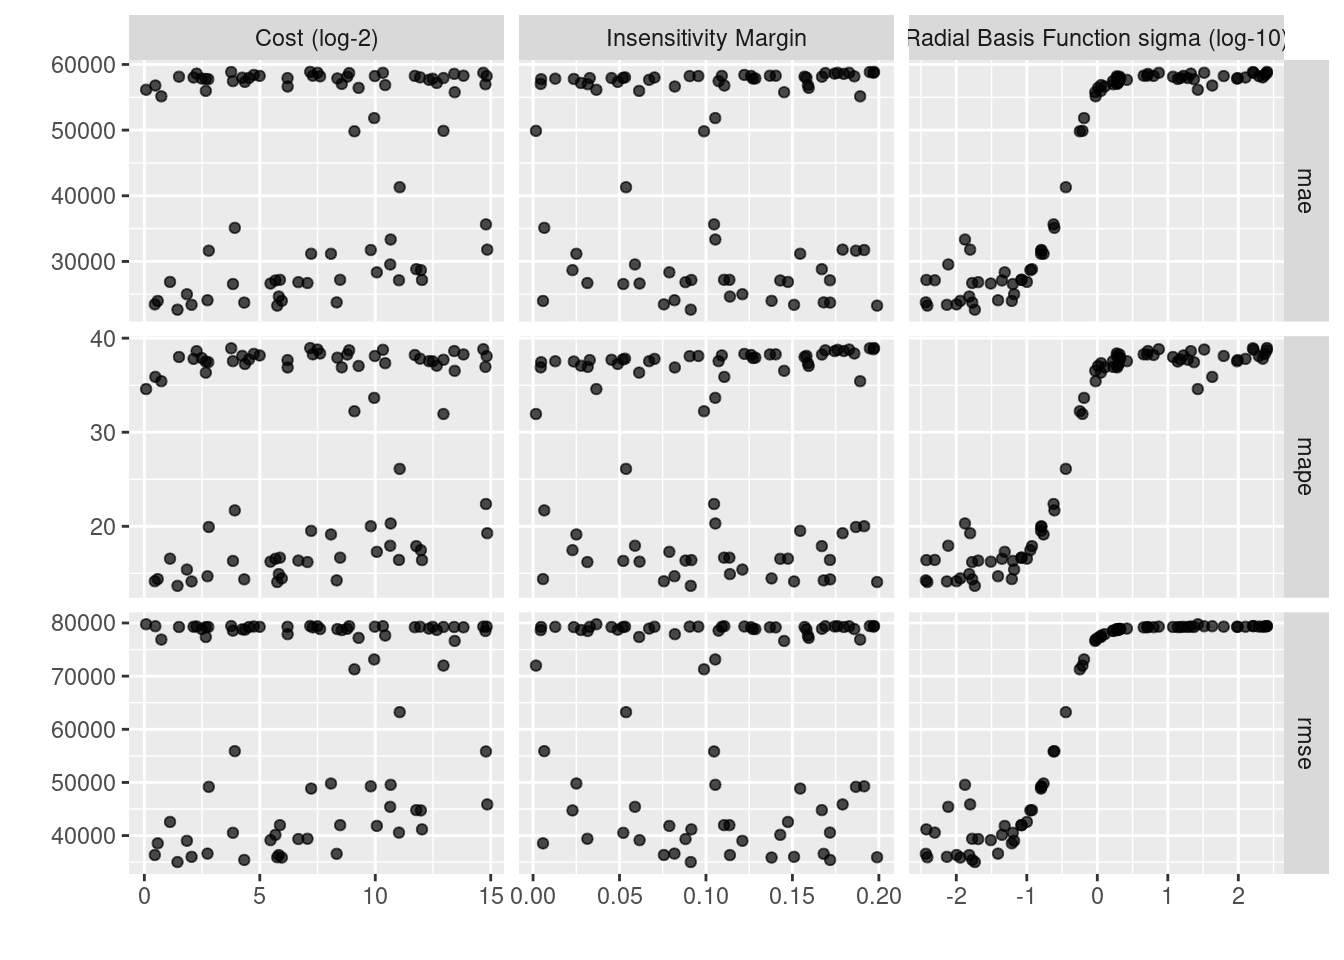
\includegraphics{amt22_03intro2mls2_files/figure-latex/unnamed-chunk-58-1.pdf}

\url{https://towardsdatascience.com/svm-and-kernel-svm-fed02bef1200}

\url{https://towardsdatascience.com/support-vector-machine-explained-8bfef2f17e71}

\url{https://medium.com/swlh/the-support-vector-machine-basic-concept-a5106bd3cc5f}

\url{https://towardsdatascience.com/unlocking-the-true-power-of-support-vector-regression-847fd123a4a0\#}:\textasciitilde:text=Support\%20Vector\%20Regression\%20is\%20a,the\%20maximum\%20number\%20of\%20points.

\url{https://www.mygreatlearning.com/blog/introduction-to-support-vector-machine/}

\url{https://www.robots.ox.ac.uk/~az/lectures/ml/lect3.pdf}

  \bibliography{book.bib,packages.bib}

\end{document}
